% Options for packages loaded elsewhere
\PassOptionsToPackage{unicode}{hyperref}
\PassOptionsToPackage{hyphens}{url}
\documentclass[
  11pt,
  oneside]{article}
\usepackage{xcolor}
\usepackage[margin=1in]{geometry}
\usepackage{amsmath,amssymb}
\setcounter{secnumdepth}{5}
\usepackage{iftex}
\ifPDFTeX
  \usepackage[T1]{fontenc}
  \usepackage[utf8]{inputenc}
  \usepackage{textcomp} % provide euro and other symbols
\else % if luatex or xetex
  \usepackage{unicode-math} % this also loads fontspec
  \defaultfontfeatures{Scale=MatchLowercase}
  \defaultfontfeatures[\rmfamily]{Ligatures=TeX,Scale=1}
\fi
\usepackage{lmodern}
\ifPDFTeX\else
  % xetex/luatex font selection
\fi
% Use upquote if available, for straight quotes in verbatim environments
\IfFileExists{upquote.sty}{\usepackage{upquote}}{}
\IfFileExists{microtype.sty}{% use microtype if available
  \usepackage[]{microtype}
  \UseMicrotypeSet[protrusion]{basicmath} % disable protrusion for tt fonts
}{}
\makeatletter
\@ifundefined{KOMAClassName}{% if non-KOMA class
  \IfFileExists{parskip.sty}{%
    \usepackage{parskip}
  }{% else
    \setlength{\parindent}{0pt}
    \setlength{\parskip}{6pt plus 2pt minus 1pt}}
}{% if KOMA class
  \KOMAoptions{parskip=half}}
\makeatother
\usepackage{longtable,booktabs,array}
\usepackage{calc} % for calculating minipage widths
% Correct order of tables after \paragraph or \subparagraph
\usepackage{etoolbox}
\makeatletter
\patchcmd\longtable{\par}{\if@noskipsec\mbox{}\fi\par}{}{}
\makeatother
% Allow footnotes in longtable head/foot
\IfFileExists{footnotehyper.sty}{\usepackage{footnotehyper}}{\usepackage{footnote}}
\makesavenoteenv{longtable}
\usepackage{graphicx}
\makeatletter
\newsavebox\pandoc@box
\newcommand*\pandocbounded[1]{% scales image to fit in text height/width
  \sbox\pandoc@box{#1}%
  \Gscale@div\@tempa{\textheight}{\dimexpr\ht\pandoc@box+\dp\pandoc@box\relax}%
  \Gscale@div\@tempb{\linewidth}{\wd\pandoc@box}%
  \ifdim\@tempb\p@<\@tempa\p@\let\@tempa\@tempb\fi% select the smaller of both
  \ifdim\@tempa\p@<\p@\scalebox{\@tempa}{\usebox\pandoc@box}%
  \else\usebox{\pandoc@box}%
  \fi%
}
% Set default figure placement to htbp
\def\fps@figure{htbp}
\makeatother
% definitions for citeproc citations
\NewDocumentCommand\citeproctext{}{}
\NewDocumentCommand\citeproc{mm}{%
  \begingroup\def\citeproctext{#2}\cite{#1}\endgroup}
\makeatletter
 % allow citations to break across lines
 \let\@cite@ofmt\@firstofone
 % avoid brackets around text for \cite:
 \def\@biblabel#1{}
 \def\@cite#1#2{{#1\if@tempswa , #2\fi}}
\makeatother
\newlength{\cslhangindent}
\setlength{\cslhangindent}{1.5em}
\newlength{\csllabelwidth}
\setlength{\csllabelwidth}{3em}
\newenvironment{CSLReferences}[2] % #1 hanging-indent, #2 entry-spacing
 {\begin{list}{}{%
  \setlength{\itemindent}{0pt}
  \setlength{\leftmargin}{0pt}
  \setlength{\parsep}{0pt}
  % turn on hanging indent if param 1 is 1
  \ifodd #1
   \setlength{\leftmargin}{\cslhangindent}
   \setlength{\itemindent}{-1\cslhangindent}
  \fi
  % set entry spacing
  \setlength{\itemsep}{#2\baselineskip}}}
 {\end{list}}
\usepackage{calc}
\newcommand{\CSLBlock}[1]{\hfill\break\parbox[t]{\linewidth}{\strut\ignorespaces#1\strut}}
\newcommand{\CSLLeftMargin}[1]{\parbox[t]{\csllabelwidth}{\strut#1\strut}}
\newcommand{\CSLRightInline}[1]{\parbox[t]{\linewidth - \csllabelwidth}{\strut#1\strut}}
\newcommand{\CSLIndent}[1]{\hspace{\cslhangindent}#1}
\setlength{\emergencystretch}{3em} % prevent overfull lines
\providecommand{\tightlist}{%
  \setlength{\itemsep}{0pt}\setlength{\parskip}{0pt}}
\usepackage{setspace}\onehalfspacing
\usepackage{placeins}
\usepackage{hyperref}
\usepackage{bbm}
\usepackage{subfig}
\usepackage{flafter}
\usepackage{booktabs}
\usepackage{longtable}
\usepackage{array}
\usepackage{multirow}
\usepackage{wrapfig}
\usepackage{float}
\usepackage{colortbl}
\usepackage{pdflscape}
\usepackage{tabularx}
\usepackage{xltabular}
\usepackage{threeparttable}
\usepackage{threeparttablex}
\usepackage[normalem]{ulem}
\usepackage{makecell}
\usepackage{xcolor}
\usepackage{siunitx}

    \newcolumntype{d}{S[
      table-align-text-before=false,
      table-align-text-after=false,
      input-symbols={-,\*+()}
    ]}
  
\usepackage{tabularray}
\usepackage[normalem]{ulem}
\usepackage{graphicx}
\usepackage{rotating}
\UseTblrLibrary{siunitx}
\NewTableCommand{\tinytableDefineColor}[3]{\definecolor{#1}{#2}{#3}}
\newcommand{\tinytableTabularrayUnderline}[1]{\underline{#1}}
\newcommand{\tinytableTabularrayStrikeout}[1]{\sout{#1}}
\usepackage{bookmark}
\IfFileExists{xurl.sty}{\usepackage{xurl}}{} % add URL line breaks if available
\urlstyle{same}
\hypersetup{
  pdftitle={Private Welfare in the Workplace},
  pdfauthor={John S. Ahlquist; Theodoros Ntounias},
  hidelinks,
  pdfcreator={LaTeX via pandoc}}

\title{Private Welfare in the Workplace}
\usepackage{etoolbox}
\makeatletter
\providecommand{\subtitle}[1]{% add subtitle to \maketitle
  \apptocmd{\@title}{\par {\large #1 \par}}{}{}
}
\makeatother
\subtitle{employee harship funds and the `substitution hypothesis'}
\author{John S. Ahlquist\footnote{Professor, School of Global Policy and Strategy, UC San Diego. \href{mailto:jahlquist@ucsd.edu}{\nolinkurl{jahlquist@ucsd.edu}}. This project was pre-registered under osf.io/fhq93. This research received grant support from the Russell Sage Foundation, UCSD's Cowhey Center for Global Transformation, and the UCSD Yankelovitch Center. Keng-Chi Chiang, Ofri Mantell, and Yuchen Wang provided research assistance. Shane Xuan assisted with Facebook.} \and Theodoros Ntounias\footnote{Postdoctoral Researcher, Skalny Center for Polish and Central European Studies, University of Rochester. \href{mailto:tntounias@pm.me}{\nolinkurl{tntounias@pm.me}}}}
\date{06 August, 2026}

\begin{document}
\maketitle

\begin{abstract}
\begin{singlespace} 

There is a long-standing claim that government social spending crowds out private savings and charity. There is also a newer set of arguments claiming that access to private resources (home equity, credit, insurance, charity) dampen voters' support for social insurance and redistributive spending. These claims have not been jointly investigated nor has the literature connected workplace programs and benefits with either outcome.  We investigate both sides of the ``substitution hypothesis'' in the context of an unstudied set of workplace private welfare programs: Employee Hardship Funds (EHFs). EHFs enable employers to distribute emergency cash to their workers using donations pooled from employees themselves. Using use three original surveys, we find that state-level variation in the social safety net is unrelated to worker support for or willingness to donate to EHFs. Experimental manipulation of EHF salience among workers at two large retailers indicates that EHFs do not displace support for public unemployment insurance or government emergency aid, regardless of the generosity of the EHF program.  Workplace-based private welfare programs like EHFs appear unconnected with government social insurance programs in the minds of workers. \\


\end{singlespace}
\end{abstract}

For centuries, pundits and scholars have debated whether government spending crowds out private savings and charity (\citeproc{ref-townsendDissertationPoorLaws1786}{Townsend 1786}; \citeproc{ref-friedmanCapitalismFreedom2002}{Friedman {[}1962{]} 2002}; \citeproc{ref-andreoniImpureAltruismDonations1990}{Andreoni 1990}; \citeproc{ref-bredtmannDoesGovernmentSpending2023}{Bredtmann 2023}; \citeproc{ref-lehmann-hasemeyerDoesSocialSecurity2018}{Lehmann-Hasemeyer and Streb 2018}). More recently, scholars of comparative political economy have studied how ``private welfare'' and ``self-insurance'' undermine support for social insurance and redistribution (\citeproc{ref-ansellPoliticalEconomyOwnership2014}{B. Ansell 2014}; \citeproc{ref-wiedemannHowCreditMarkets2022}{Wiedemann 2022}; \citeproc{ref-ahlquistTakingCreditRedistribution2017}{Ahlquist and Ansell 2017}; \citeproc{ref-prasadLandTooMuch2012}{Prasad 2012}; \citeproc{ref-busemeyerWelfareStatePrivate2020}{Busemeyer and Iversen 2020}). Almost entirely absent from these discussions are large firms, which have tremendous leeway to introduce, revise, and eliminate employee health and life insurance coverage, retirement programs, transportation and childcare subsidies, and charitable initiatives. Does employer-based ``private welfare'' feed back into the political system, reducing support for government spending on these same activities? Does government welfare effort affect worker interest in firm-driven private welfare and charitable programs?

In this paper, we focus on one unstudied type of workplace program that combines \emph{both} private welfare and charitable activities: Employee Hardship Funds (EHFs). These now-widespread programs---operating largely in the US---are set up by corporations as tax-exempt charities. Employers solicit donations from their own employees to fund cash grants to their workers during times of unexpected personal hardship. As essentially scaled up, tax-advantaged versions of ``passing the hat,'' EHFs echo the long tradition of worker mutual aid. We use them to study both directions of the ``substitution hypothesis.'' As a form of corporate charitable activity, we can examine whether worker interest in and donation to EHF programs varies as a function of government welfare effort. As a form of private welfare, we can examine whether EHF salience affect workers' support for government programs to aid the unemployed and those in need.

We fielded three pre-registered surveys. In Study 1, an original survey of US retail workers, we ask whether variation across US States in welfare effort predicts worker interest in and willingness to donate to EHFs. In Study 2 and 3, we fielded two original, independent surveys of workers at two large US retailers with long-standing EHF programs of widely differing generosity. We experimentally manipulate worker awareness of their employer's EHF by randomly assigning some workers to watch employer-produced or adapted testimonial videos from EHF grant recipients. We ask whether exposure to these messages about a form of private welfare affects support for government programs aiding the unemployed and those in need.\footnote{A companion paper (\citeproc{ref-ahlquistPrivateWelfareWorkplace2026}{\textbf{ahlquistPrivateWelfareWorkplace2026?}}) uses these same underlying data to study different outcomes: job attachment and unionization interest. Because both papers rely on the same programs, surveys, and experiments, we necessarily share some description of EHFs, case selection, and research design; we keep that material to the minimum needed here and refer readers to (\citeproc{ref-ahlquistPrivateWelfareWorkplace2026}{\textbf{ahlquistPrivateWelfareWorkplace2026?}}) for the fullest account of program histories, recruitment, and measurement.} In the end, we find that our EHF treatments do \emph{not} reduce support for government social insurance among workers at either firm, regardless of program generosity. Even though our EHF treatment increases worker willingness to donate to the EHF, this effect is not moderated by state-level welfare generosity or individual-level considerations such as religiosity and partisanship. Using hierarchical models, we also find no detectable relationship between state-level welfare regimes and broader worker interest in EHF programs. Taken together, these findings suggest that EHFs and government social insurance programs are unconnected in the minds of workers. In short, we find no evidence consistent with either version of the substitution hypothesis with respect to workplace programs.

Our findings make five contributions. First we highlight how workplace benefits have been excluded from broader debates about private welfare and the crowd out between government spending and private initiatives. Second, we show how researchers can exploit variation in workplace benefits to speak to broader social science debates. Third, we highlight EHFs as curious, understudied workplace programs. Fourth, in the case of EHFs, we fail to uncover evidence that this workplace program connects meaningfully with political attitudes. This lack of connection may be because EHFs are too new or too small to matter, but future research will be needed. Finally, there are policy stakes. EHFs connect to several areas of concern in the contemporary American political economy, including notable inequities across workers as well as increased employer leverage over workers in an era of monopsonistic local labor markets, weak unions, and strained safety nets. For example, EHFs, as with all workplace benefits, are conditional on employment with a specific firm, potentially exacerbating inequality across workers at different firms or in different sectors. EHFs may also increase employer power over workers when they are most vulnerable, similar to the ``welfare capitalism'' of the past (\citeproc{ref-brandesAmericanWelfareCapitalism1976}{Brandes 1976}; \citeproc{ref-jacobyModernManorsWelfare1998}{Jacoby 1998}). EHFs, as with many job-related benefits, lack formal mechanisms for worker input and accountability, beyond worker quits. On the positive side, workers appear to value emergency aid and corporations may be more efficient at delivering immediate cash assistance than governments, at least to the families of the employed.

In the next section we go into both forms of the substitution hypothesis in more detail, highlighting the absence of any real consideration of workplace programs and benefits. Section \ref{sec-ehf-bkgrnd} provides the necessary background on EHFs and summarizes the main hypotheses we examine here. Section \ref{sec-genpop} describes the research design and results for Study 1 while Section \ref{sec-study2-3} describes the case selection, survey experiments, and results from Studies 2 and 3. Section \ref{sec-conclusion} concludes.

\section{The ``substitution hypothesis,'' two ways}\label{sec-lit}

This paper builds on two largely disconnected literatures concerned with whether private resources and public welfare or social insurance substitute for one another. The first literature stems from arguments emerging as far back as the 18th Century (at least), claiming that government spending on poverty relief, welfare, and social insurance crowds out private charitable giving and private savings. The second and more recent literature works in the opposite direction. It focuses on the links between improved access to private financial resources---credit, appreciating assets, insurance---and reduced voter support for public welfare and social insurance programs. Both of these versions of the substitution hypothesis bear some resemblance to the policy feedback literature, long a staple of American politics, in which ``policies make politics'' (\citeproc{ref-schattschneiderPoliticsPressureTarriff1935}{Schattschneider 1935}; \citeproc{ref-campbellPolicyMakesMass2012}{Campbell 2012}). Nevertheless, the substitution hypothesis literatures we draw on are less concerned with how government policies create organized constituencies to reinforce or undermine that policy. Importantly, none of these various strands of thought has looked squarely at whether workplace benefits and charitable programs might relate to voter attitudes toward government welfare efforts.

\subsection{Government spending crowds out private savings and charity}\label{government-spending-crowds-out-private-savings-and-charity}

Almost as soon as governments began systematically spending tax money in support of the poor, aged, and infirm, arguments emerged that such spending is actually counterproductive.\footnote{Defoe (\citeproc{ref-defoeGivingAlmsNo1893}{{[}1704{]} 1893}) is the first we could uncover in the British tradition.} The reasons given often had much to do with purported moral failings among the laboring classes, but political economy arguments eventually emerged. Townsend (\citeproc{ref-townsendDissertationPoorLaws1786}{1786}) may have been the first to articulate the claim that tax-funded social spending will depress \emph{both} private savings and private charity.\footnote{Townsend says ``Let the same {[}generous, charitable{]} man be straitened in his circumstances, let him be burthened with taxes\ldots and he will have little inclination to seek for objects of distress, or to visit the sequestered cottage of the silent sufferer\ldots If, agreeable to the general practice of the labouring poor, a man\ldots has made no provision for his future wants; if all, to whom he might naturally look for aid, are in the same circumstances with himself; and if the charity of those among his neighbours, who are distinguished for benevolence, nay of all who have the common feelings of humanity, is exhausted; if they who are most willing are least able to relieve him; we must expect to see distress and poverty even among those who are worthy of compassion.''} Malthus (\citeproc{ref-malthusEssayPrinciplePopulation1798}{1798}) claims that ``The poor laws of England may therefore be said to diminish both the power and the will to save among the common people'' (Ch. 5). de Tocqueville (\citeproc{ref-detocquevilleAlexisTocquevillesMemoir1997}{{[}1835{]} 1997}) created a distinction between ``private'' and ``legal'' charity, arguing in favor of the former over the latter.\footnote{He states that ``any permanent, regular, administrative system whose aim will be to provide for the needs of the poor, will breed more miseries than it can cure, will deprave the population that it wants to help and comfort, will in time reduce the rich to being no more than the tenant-farmers of the poor, will dry up the sources of savings, will stop the accumulation of capital, will retard the development of trade, will benumb human industry and activity, and will culminate by bringing about a violent revolution in the State, when the number of those who receive alms will have become as large as those who give it, and the indigent, no longer being able to take from the impoverished rich the means of providing for his needs, will find it easier to plunder them of all their property at one stroke than to ask for their help.''}

As the welfare state expanded dramatically in the post-War period, these arguments revived (\citeproc{ref-friedmanCapitalismFreedom2002}{Friedman {[}1962{]} 2002}), along with empirical scrutiny. Feldstein (\citeproc{ref-feldsteinSocialSecurityInduced1974}{1974}) argued that Social Security depressed household private savings by 30-50\%, spawning an ongoing debate about the scale of substitution and its consequences (\citeproc{ref-alessiePensionWealthHousehold2013}{Alessie, Angelini, and van Santen 2013}; \citeproc{ref-lehmann-hasemeyerDoesSocialSecurity2018}{Lehmann-Hasemeyer and Streb 2018}). Several theoretical models, based on the assumption that charities provide public goods, imply that government spending will crowd out private charity to some degree (\citeproc{ref-andreoniImpureAltruismDonations1990}{Andreoni 1990}; \citeproc{ref-warrParetoOptimalRedistribution1982}{Warr 1982}; \citeproc{ref-bergstromPrivateProvisionPublic1986}{Bergstrom, Blume, and Varian 1986}). Subsequent empirical work focused on determining whether government spending crowds out private giving dollar-for-dollar (as in models of ``pure altruism'') or at some lesser rate (``impure altruism''). A variety of empirical contexts and research designs produced widely varying estimates, including some evidence of ``crowding in'' (\citeproc{ref-dewitGovernmentSupportCharitable2016}{De Wit and Bekkers 2016}; \citeproc{ref-bredtmannDoesGovernmentSpending2023}{Bredtmann 2023}; \citeproc{ref-andreoniCharitableGiving2013}{Andreoni and Payne 2013}).\footnote{Crowding-in is most frequently observed in studies of government grants to specific charities, in which government support may signal need or charity quality, a line of reasoning irrelevant to this paper. A more relevant possibility is that both government spending and private charity are signals (or byproducts) of broader cultural or institutional dispositions toward collective support (\citeproc{ref-dewitGovernmentExpendituresShift2018a}{De Wit et al. 2018}). Lab experimental studies tend to provide the largest estimates of crowding out.} The weight of evidence suggests that government spending \emph{can} crowd out some proportion of charity and savings, but the scale is unclear and the details matter.

Most relevant to this study, Hungerman (\citeproc{ref-hungermanAreChurchState2005a}{2005}) and Gruber and Hungerman (\citeproc{ref-gruberFaithbasedCharityCrowdout2007}{2007}) exploit variation across US States in spending for social support, estimating that government social welfare spending reduces charitable relief from churches by about 30\%. Paarlberg et al. (\citeproc{ref-paarlbergPoliticsDonationsAre2019}{2019}) lack an identification strategy, but find that counties with lower tax burdens and higher proportions of Republican voters also donate more to charity. In some of the more well-identified studies, charitable organizations take in donations and then provide services. This complicates interpretation as fundraising effort responds strategically to government support (\citeproc{ref-andreoniCrowdingOutDue2011}{Andreoni and Payne 2011}). Panjwani and Xiong (\citeproc{ref-panjwaniCausesConsequencesMedical2023}{2023}) show that health-related crowdfunding campaigns (i.e., demand for charity) declined after expansions in medical insurance coverage due to the Affordable Care Act. Lee and Lehdonvirta (\citeproc{ref-leeNewDigitalSafety2022}{2022}) show that areas with poor private insurance coverage and fewer social associations see greater crowdfunding campaign initiation rates, but campaigns in these same areas are \emph{less} likely to be successful (i.e., charitable capacity or norms might be weaker). Bernard and Gazel (\citeproc{ref-bernardOutCrowdingEffects2025}{2025}) show that crowdfunding projects with low excludability (i.e., you do not need to donate to enjoy benefits, should the project go forward) exhibit the most crowding out. EHFs are non-excludable in this regard.

In attempting to estimate the crowd out rate, existing empirical work often relies actual government social spending as the measure of effort, as opposed to indicators of the spending ``regime'' (\citeproc{ref-esping-andersenThreeWorldsWelfare1990}{Esping-Andersen 1990}). This is a problematic conflation for at least three reasons. First, spending levels at any point in time are endogenous to conditions that may also affect savings and charitable giving.\footnote{There are several clever empirical strategies for addressing this, but they produce different estimates of crowd out from very different contexts (\citeproc{ref-boberg-fazlicDoesWelfareSpending2017}{Boberg-Fazlić and Sharp 2017}; \citeproc{ref-hungermanAreChurchState2005a}{Hungerman 2005}; \citeproc{ref-gruberFaithbasedCharityCrowdout2007}{Gruber and Hungerman 2007}; \citeproc{ref-andreoniGrantsCharitiesCrowd2014}{Andreoni, Payne, and Smith 2014})} Second, citizens' beliefs about government spending in specific areas are only weakly connected to actual spending levels (which fluctuates more than opinion) (\citeproc{ref-dewitHeterogeneityCrowdingoutWhen2017}{De Wit, Bekkers, and Broese van Groenou 2017}). Voter knowledge about the level of government support directed to particular intermediary charities is even more meager (\citeproc{ref-horneCharitableDonorsKnow2005}{Horne, Johnson, and Van Slyke 2005}). Voter beliefs about government spending levels, however, are connected to their pre-existing partisan identities (\citeproc{ref-bullockPartisanBiasFactual2015}{Bullock et al. 2015}; \citeproc{ref-mettlerSubmergedState2011}{Mettler 2011}). Klein Teeselink and Melios (\citeproc{ref-kleinteeselinkPartisanshipPoliticalAlignment2025}{2025}) show that co-partisans of the US President reduce their charitable donations independently of any changes to the level and composition of actual spending, likely because they are more confident in the efficacy of government when their preferred party is in power. Third, expectations about the adequacy of \emph{future} spending should matter when forming opinions or making donations. As such, the adequacy and credibility of social spending \emph{regimes} would be more relevant than actual spending levels at any moment in time, as Esping-Andersen (\citeproc{ref-esping-andersenThreeWorldsWelfare1990}{1990}) noted decades ago.\footnote{``Expenditures are epiphenomenal to the theoretical substance of welfare states.'' p.19} We take this seriously in our measurement choices below.

Firms are significant sources of charitable funding across a range of causes. Firm-directed funding can take the form of corporate donations to specific charities or even individuals. But firms also actively organize their employees to donate their private resources, sometimes using matching or other incentives (\citeproc{ref-meierSubsidiesIncreaseCharitable2007}{Meier 2007}). Firms appear to give for different reasons than individuals (\citeproc{ref-brammerCorporateReputationPhilanthropy2005}{Brammer and Millington 2005}; \citeproc{ref-bertrandHallMirrorsCorporate2021}{Bertrand et al. 2021}), but workplace philanthropic fundraising is significant (\citeproc{ref-rimesGivingWorkExploring2019}{Rimes, Nesbit, and Christensen 2019}; \citeproc{ref-shakerGiveOfficeReview2019}{Shaker and Christensen 2019}). Political scientists have studied employer-organized political donations (\citeproc{ref-hertel-fernandezPoliticsWork2018}{Hertel-Fernandez 2018}; \citeproc{ref-stuckatzHowWorkplaceAffects2022}{Stuckatz 2022}), which do appear to partially crowd out other charitable contributions (\citeproc{ref-yildirimArePoliticalCharitable2024}{Yildirim et al. 2024}). But, as yet, there is no work examining any link between the government safety net and workplace giving, especially when the beneficiaries of workplace charity are other workers. We provide the first such test looking at EHF programs.

\subsection{Private resources crowd out support for a public safety net}\label{private-resources-crowd-out-support-for-a-public-safety-net}

A newer, smaller, and largely parallel literature has emerged, documenting how shocks to private resources affect voter support for public social programs. Most obviously, governments sometimes step in when private resources are diminished. Margalit (\citeproc{ref-margalitExplainingSocialPolicy2013}{2013}) uses panel data around the Great Recession and finds that people who lose their job become more supportive of government support for the unemployed, but when the need dissipates, so does their support for government unemployment insurance, especially among Republican voters. As an historical matter, government administered, tax-funded unemployment insurance grew out of the repeated collapse (and ad hoc bailouts) of privately-organized welfare and mutual aid pools (\citeproc{ref-socialsecurityadministrationSocialSecurityHistory2023}{Administration 2023}; \citeproc{ref-westernClassMarketPrinceton1997}{Western 1997}).

Recently, scholars have asked whether improvements in private resources can crowd out support for government social insurance and welfare programs. The logic is simple: voters who perceive an improved financial position are more confident in their ability to ``self-insure'' against negative income shocks while also becoming less willing to pay taxes into the public system from which they perceive a reduced benefit. Real estate (especially housing) is a key, politically relevant asset and source of savings (\citeproc{ref-ansellPoliticsHousing2019}{B. W. Ansell 2019}). B. Ansell (\citeproc{ref-ansellPoliticalEconomyOwnership2014}{2014}) finds that American and British voters with appreciating real estate assets are less supportive of social insurance. Wiedemann (\citeproc{ref-wiedemannHowCreditMarkets2022}{2022}) and Ahlquist and Ansell (\citeproc{ref-ahlquistTakingCreditRedistribution2017}{2017}) focus on easy access to credit (related to home ownership and real estate prices) as a key private resource that can reduce pressure for redistributive policy and social spending. Where real estate is more financialized (i.e., more tied to credit markets), home owners are less supportive of redistributive social policies (\citeproc{ref-andreHomeOwnershipSupport2016}{André and Dewilde 2016}).

Beyond housing and credit, economic risk and access to insurance has been a major area of interest. Those able to ``self-insure'' through higher wealth and incomes are less worried about negative economic shocks and less supportive of government spending to help the unemployed, infirm, and aged (\citeproc{ref-rehmInsecureAlliancesRisk2012}{Rehm, Hacker, and Schlesinger 2012}; \citeproc{ref-hackerInsecureAmericanEconomic2013}{Hacker, Rehm, and Schlesinger 2013}). Busemeyer and Iversen (\citeproc{ref-busemeyerWelfareStatePrivate2020}{2020}) provide a theoretical account and empirical data illustrating how the presence of private insurance options reduces high-income voters' support for unemployment and pension spending. Increasingly fine-grained data combined with growing income inequality increase the scope for private insurance options to emerge, weakening support for ``solidaristic'' government policies (\citeproc{ref-iversenBigDataWelfare2022}{Iversen and Rehm 2022}).\footnote{Hadziabdic and Kohl (\citeproc{ref-hadziabdicPrivateSpannerPublic2022}{2022}), using German panel data, finds no robust relationship between taking out life insurance and broad attitudes around social spending and government activity.}

Private charity is also relevant here. Werfel (\citeproc{ref-werfelDoesCharitableGiving2018}{2018}) uses survey experiments to manipulate beliefs about the degree of private charitable funding directed at specific needs. In the area of social services, greater perceived charitable activity significantly reduced support among conservatives and moderates for government spending in that same area.

Again, however, there is a dearth of research that explores how variation in employer-provided amenities and insurance as well as corporate charitable efforts affect voter attitudes and behavior. This is remarkable, as there is considerable variation across firms and over time and space in workplace amenities as well as corporate charitable initiatives. Insofar as EHFs are a form of private emergency aid, increased program awareness could blunt support for social insurance or government aid programs in times of emergency (e.g., COVID-19). This paper seeks to determine whether we can observe this effect among US retail workers.

\section{Employee Hardship Funds}\label{sec-ehf-bkgrnd}

\subsection{Background}\label{background}

In the contemporary United States, unions are vanishing and the welfare and social insurance systems are strained. Temporary and other ``non-standard'' work arrangements have spread (\citeproc{ref-abrahamMeasuringGigEconomy2021}{Abraham et al. 2021}; \citeproc{ref-weilFissuredWorkplace2014}{Weil 2014}) without providing access to traditional social insurance and labor-market protections (\citeproc{ref-thelenAmericanPrecariatCapitalism2019}{Thelen 2019}). Americans in the lower half of the education and earnings distributions have seen wages stagnate even as they bear more economic risk (\citeproc{ref-hackerGreatRiskShift2019}{Hacker 2019}).

Against this backdrop, many US employers have set up programs ostensibly designed to provide emergency aid to their workers. For example, two of the largest retailers in the world, the Home Depot and Walmart maintain, respectively, the Homer Fund and Associates in Critical Need Trust (ACNT).\footnote{ACNT has since been renamed the ACNT Together Fund.} Both programs are incorporated as non-profit charities (501(c)(3)) that make cash grants to employees facing emergency expenses. These grants are funded by tax-deductible donations solicited directly from corporate and front-line employees alike; grants to workers are tax-exempt. We describe the two programs, which differ substantially in generosity and promotion, in Section \ref{sec-study2-3}.

The Homer Fund and ACNT are examples of \emph{Employee Hardship Funds} (EHFs), which blend features of charity with the job amenities of private ``welfare capitalism''. Workers are both asked to donate to these funds while hearing that their employer intends to help in times of unexpected hardship. Moreover, the structure and generosity of these programs varies significantly across employers.

Despite operating at hundreds of large firms, EHFs remain virtually unstudied outside a small practitioner literature (\citeproc{ref-associationofdisasterrelieffundsandemployeehardshipfundsEnvironmentalScanDisaster2013}{Association of Disaster Relief Funds and Employee Hardship Funds 2013}; \citeproc{ref-employeerelieffundeducationgroupEnvironmentalScanDisaster2019}{Group 2019}; \citeproc{ref-aspeninstituteIlluminatingHiddenSafety2019}{Institute 2019}; \citeproc{ref-rodriguezEmployeeHardshipFunds2020}{Rodriguez 2020b}, \citeproc{ref-rodriguezEveryCompanyShould2020}{2020a}),\footnote{Amorim and Schneider (\citeproc{ref-amorimScheduleUnpredictabilityHighCost2022}{2022}) and Reich and Bearman (\citeproc{ref-reichWorkingRespectCommunity2018}{2018}) are the only peer-reviewed pieces we know of that even mention EHFs.} There is no central registry exists. We have nonetheless documented over 320 firms across many sectors operating EHFs as of January 2025, including nine of the ten largest US retailers by revenue. Corporate interest in EHFs has been sufficient to support a cottage industry of third-party entities that create and manage EHFs on behalf of their clients. The largest of these appears to be the Employee Assistance Foundation (EAF), which reports over 400 corporate clients and distributed more than \$86 million in grants in 2020.

EHF activity appears to be growing. Levi Strauss reported a threefold rise in EHF applications in 2020 (\citeproc{ref-rodriguezEveryCompanyShould2020}{Rodriguez 2020a}), with a further spike once federal pandemic aid lapsed, and EAF reported more than a tenfold jump in applications over historical averages in the first half of 2020 alongside 140 new client programs (\citeproc{ref-employeeassistancefoundationDecadeAssistanceOffering2022}{Foundation 2022}). Home Depot suspended employee fundraising and expedited grants during the pandemic. In May 2020, amid criticism of its workplace-safety record and nascent unionization at its warehouses, Amazon launched a \$25 million EHF, which it closed in August 2022.

Figure \ref{fig:fig-HfACNTcomps} compares the Home Depot and Walmart programs using IRS Form 990 data. The left panel plots net assets of each firm's nonprofit foundation;\footnote{For tax purposes each EHF sits within the larger Home Depot and Walmart corporate foundation, respectively.} both grew strongly after 2010, but the Homer Fund runs at more than double ACNT's size. The right panel plots grants to domestic individuals, our preferred measure of EHF activity.\footnote{Large foundations mostly disburse to other nonprofits rather than individuals. The Homer Fund website reports \$17 million in 2023 EHF grants against the \$19.1 million in individual grants in the Home Depot foundation's 2023 Form 990.} The Homer Fund made \$15--25 million in annual individual grants between 2008 and 2022, versus typically under \$10 million for ACNT, despite Walmart's far larger workforce. Over their lifetimes the Homer Fund reports more than \$267 million to over 183,000 individuals and ACNT more than \$142 million to over 145,000.

\begin{figure}

\includegraphics[width=0.5\linewidth]{Ahlquist_Ntounias_EHF_SI_2026_files/figure-latex/fig-HfACNTcomps-1} 
\includegraphics[width=0.5\linewidth]{Ahlquist_Ntounias_EHF_SI_2026_files/figure-latex/fig-HfACNTcomps-2} \caption{EHF assets and grant activity at the Home Depot and Walmart.}\label{fig:fig-HfACNTcomps}
\end{figure}

These two programs illustrate a broader pattern: EHFs differ across firms on nearly every dimension---longevity, eligibility, generosity, funding, administration, and the intensity of employer promotion---variation we exploit in Studies 2 and 3.

\subsection{Hypotheses}\label{hypotheses}

Connecting EHFs to both forms of the substitution hypothesis is straightforward. If the first form of the substitution hypothesis holds, we expect workers in places with stronger government safety nets to be less interested in and less willing to donate to EHFs. Existing work also suggests that political conservatives may be more attentive to these ostensible trade-offs. In the US, there is considerable variation across states in the generosity of unemployment and welfare benefits as well as in the administrative burdens workers face in accessing benefits when needed. We exploit this cross-state variation below.

In the other direction, workers exposed to information about their employer's EHFs should see that they have access to additional resources should they encounter certain emergencies. As their employer is now intervening, workers will be less supportive of government programs to support people in times of hardship. The more generous the EHF, the less a worker may perceive a need for public programs.

We collect these hypotheses in Table \ref{tab:tab-hypotheses} for ease of reference.

\begin{table}[!h]
\centering
\caption{\label{tab:tab-hypotheses}Summary of Empirical Hypotheses}
\centering
\begin{tabular}[t]{l>{\raggedright\arraybackslash}p{10cm}l}
\toprule
Hypothesis & Description & Study\\
\midrule
\cellcolor{gray!10}{H1} & \cellcolor{gray!10}{Workers in states with more generous social spending regimes will be less supportive of EHFs and less willing to donate.} & \cellcolor{gray!10}{1, 3}\\
H1a & The correlation with state spending will be stronger among conservatives & 1\\
\cellcolor{gray!10}{H2} & \cellcolor{gray!10}{Exposure to EHF messaging reduces support for government spending on social insurance and welfare.} & \cellcolor{gray!10}{2, 3}\\
H2a & Effects should be bigger among those unaware of the EHF before treatment. & 2, 3\\
\cellcolor{gray!10}{H2b} & \cellcolor{gray!10}{Effects should be bigger where the EHF is more generous.} & \cellcolor{gray!10}{2, 3}\\
\bottomrule
\end{tabular}
\end{table}

\section{Study 1}\label{sec-genpop}

Study 1 addresses H1 and H1a. We fielded an original survey of US retail workers probing their knowledge of and experience with EHFs---whether their employer offers one, and how much they support such programs. Concentrating on a single industry holds cross-industry variation fixed. Retail is a natural choice: it employs over 15 million Americans, a number that has grown over the past decade, and is characterized by low wages, limited human-capital investment, and unpredictable scheduling---conditions under which EHF-style benefits might be especially valued.

The survey ran on the CloudResearch incentivized panel, targeting US retail workers aged 18 and over, in the field 12--22 February 2025, yielding 1008 valid responses.\footnote{Following our pre-registratioin, we analyze only respondents with US IP addresses who passed a retail-employment screen and two attention checks; duplicate IP addresses reporting identical demographics were also excluded.} Using 2024 American Community Survey demographics for US retail workers, we built post-stratification weights on gender, race, and education. Sample descriptives appear in Appendix \ref{app-genpop-survsum}.

\subsection{Research design}\label{research-design}

In the US, virtually all social safety net and labor market benefits for working age citizens are managed at the state level.\footnote{Social Security, Medicare, and veterans' benefits are the primary programs that are run directly by the federal government.} Consequently, there is significant variation across states in both the generosity of the social safety net and the ease of accessing the benefits that are available (\citeproc{ref-herdAdministrativeBurdenPolicymaking2019}{Herd and Moynihan 2019}; \citeproc{ref-foxEffectAdministrativeBurden2023}{Fox, Feng, and Reynolds 2023}). For example, in normal economic times, most states offer up to 26 weeks of unemployment insurance benefits, with some states offering as little as 12 while Montana provides 28. The main cash welfare program, Temporary Assistance to Needy Families (TANF), provides a maximum monthly benefit of \$915 in New Hampshire but only \$162 in Arkansas for a single parent of one child of in 2023 (\citeproc{ref-falkTemporaryAssistanceNeedy2024}{Falk and Landers 2024}).

In Study 1, we rely on cross-state variation in the robustness of their social safety nets to look at two specific outcomes: the degree of support for an EHF at the respondent's current retail employer and the stated willingness to donate to the EHF. Both outcomes are ordered categorical variables.\footnote{Outcome categories for the donation question were \{nothing at all, one time donation less than \$20, one time donation more than \$20, regular donation of less than \$20, regular donation of more than \$20\}.} Question wording varied slightly based on whether a respondent reported an employer with an EHF so we condition on whether the respondent claims to have an EHF.\footnote{We were not in a position to verify whether respondent reports were accurate, so this represents perceptions only.}

In measuring variation in the state-level safety net, we rely on the standardized benefit levels produced by Schmidt, Shore-Sheppard, and Watson (\citeproc{ref-schmidtStateSafetyNet2024}{2024}). In our main specifications, we use the ``state directed'' portion of these benefits, to better isolate differences across states.\footnote{Our findings do not hinge on this decision. Using the ``cash and food'' benefits estimates in Schmidt, Shore-Sheppard, and Watson (\citeproc{ref-schmidtStateSafetyNet2024}{2024}) or the measure of TANF benefit generosity from Fox, Feng, and Reynolds (\citeproc{ref-foxEffectAdministrativeBurden2023}{2023}) produce similar results. Measure of UI generosity, including maximum weeks of benefits and average weekly benefit amounts also show no relationship with EHF support or donation.}

\subsection{Results}\label{results}

Figure \ref{fig:fig-ehf-genretail} displays the distributions of both EHF outcomes against safety net generosity, measured in US dollars. Inspection of the graphs suggests that there is no relationship between safety net generosity and either support for or willingness to donate to an EHF.

\begin{figure}

{\centering \subfloat[Support\label{fig:fig-ehf-genretail-1}]{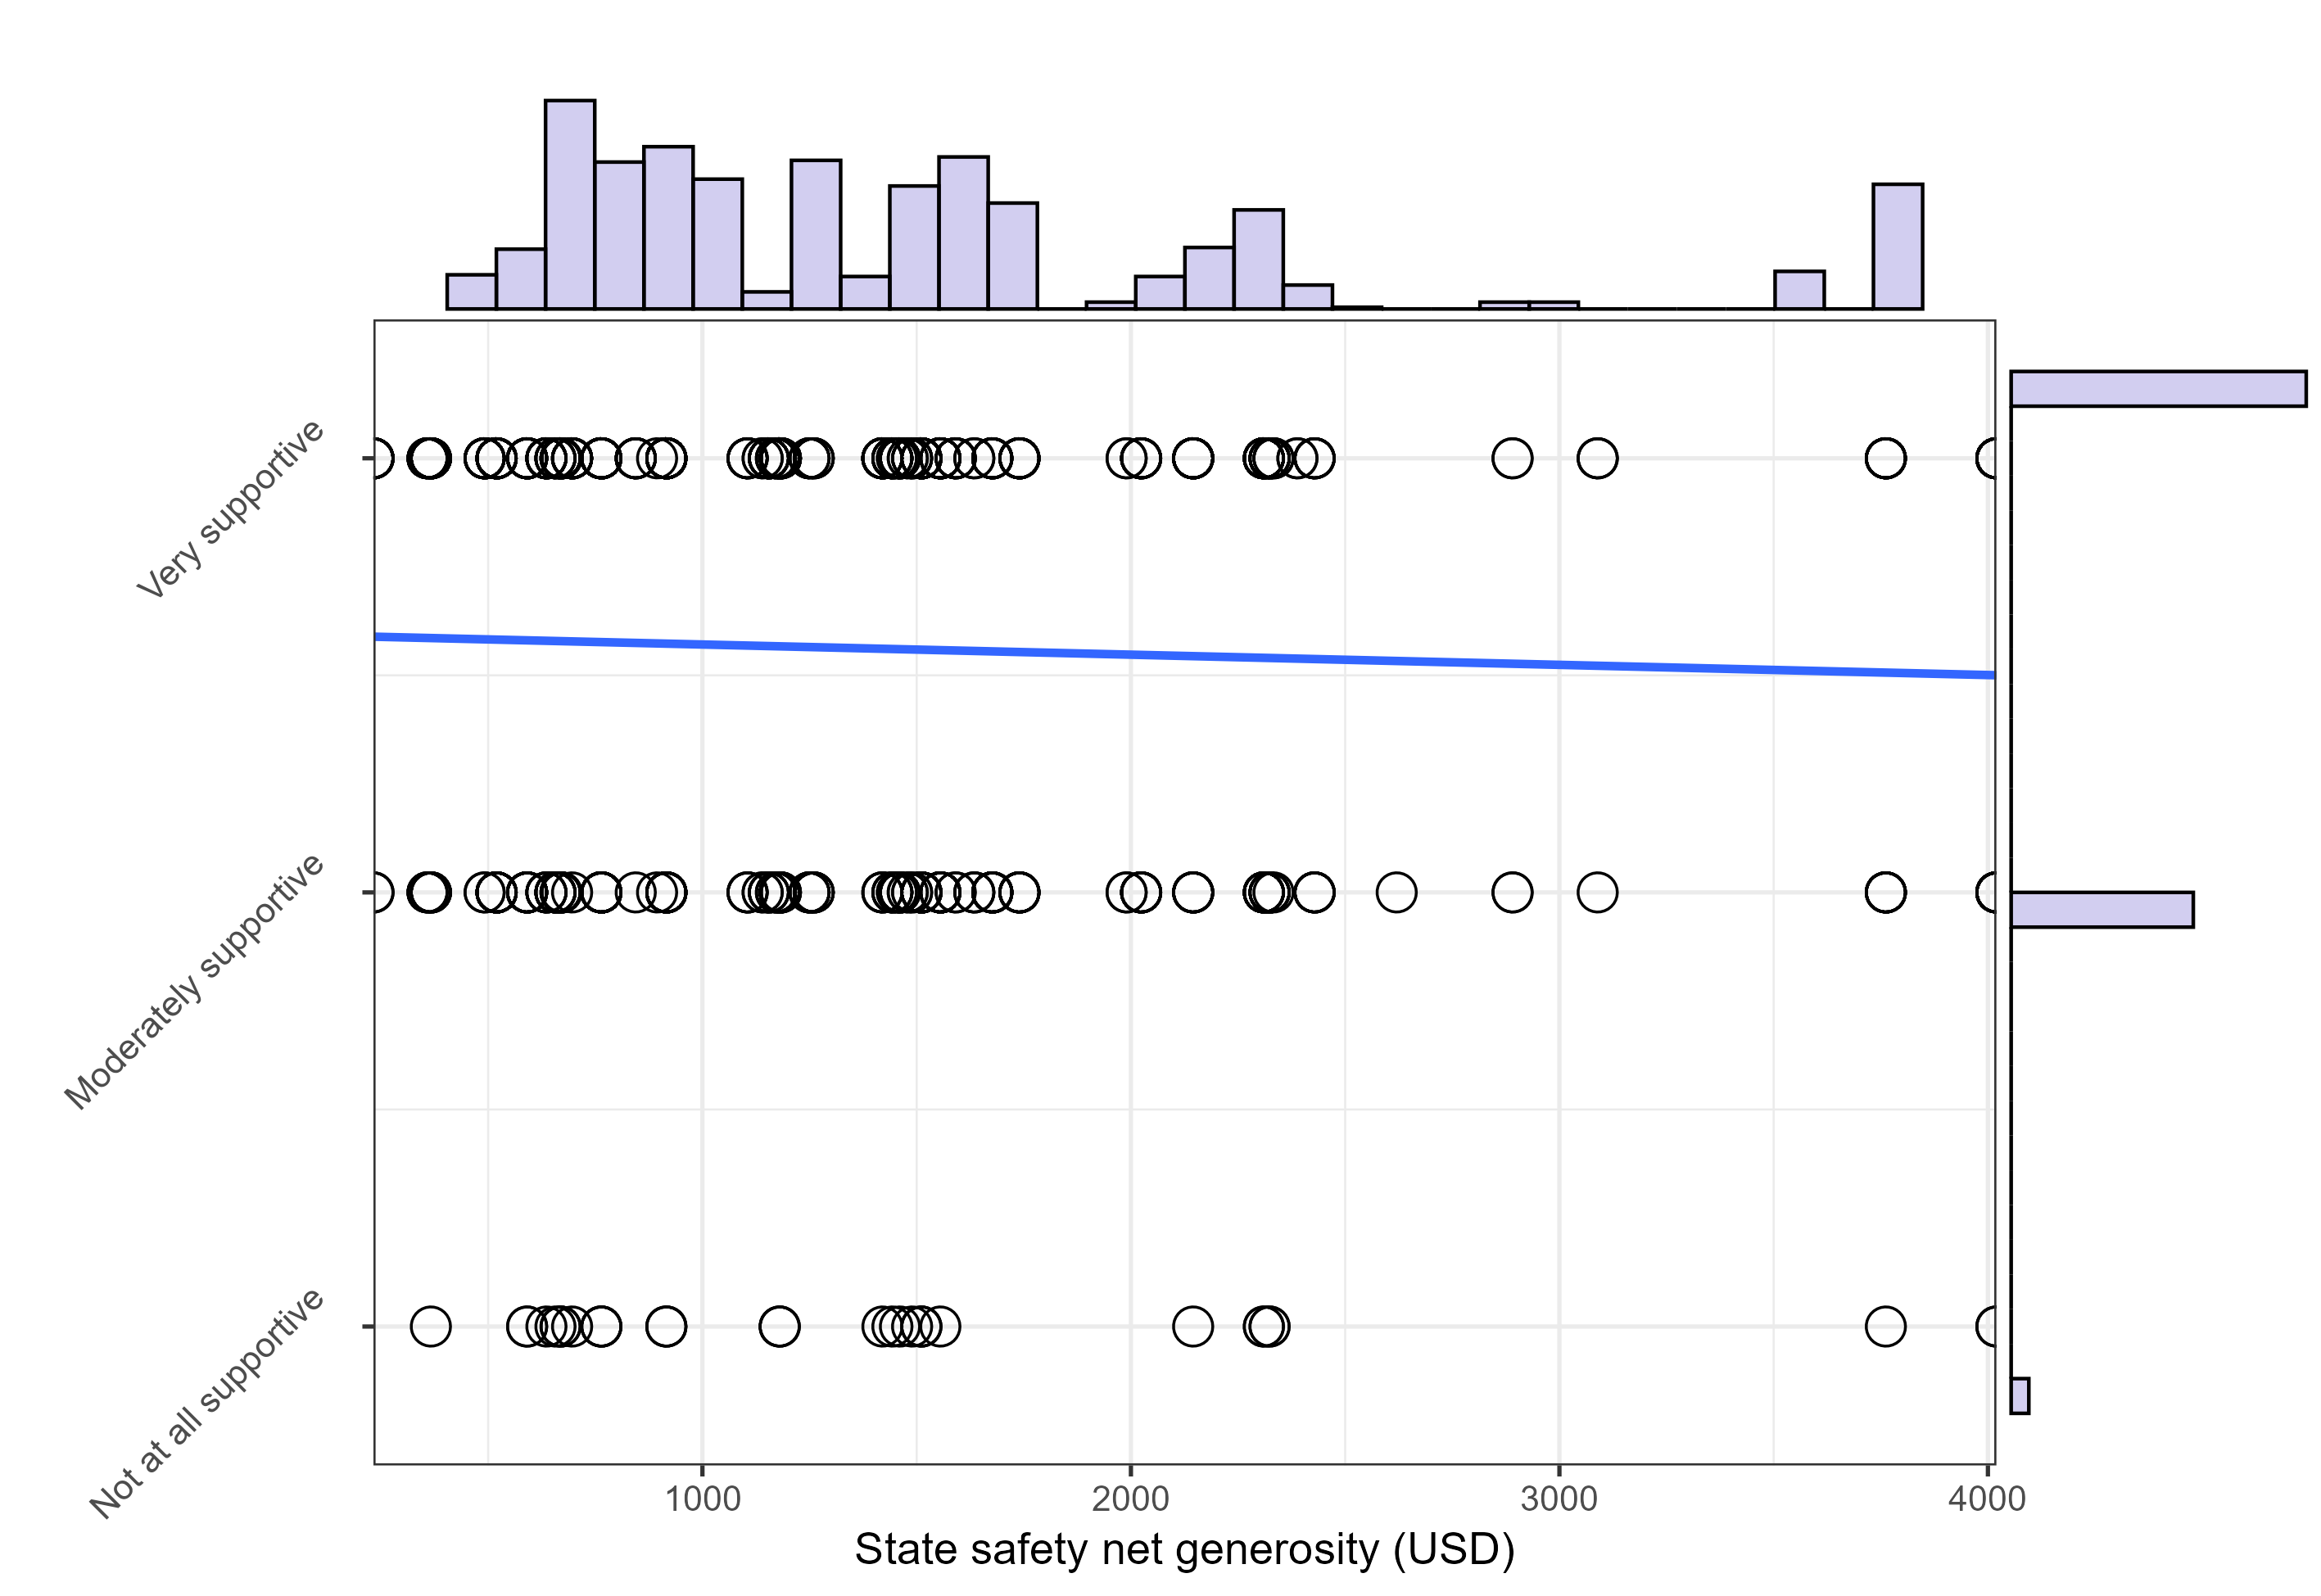
\includegraphics[width=0.5\linewidth]{../plots/ui_plot_gr_supp} }\subfloat[Willingness to Donate\label{fig:fig-ehf-genretail-2}]{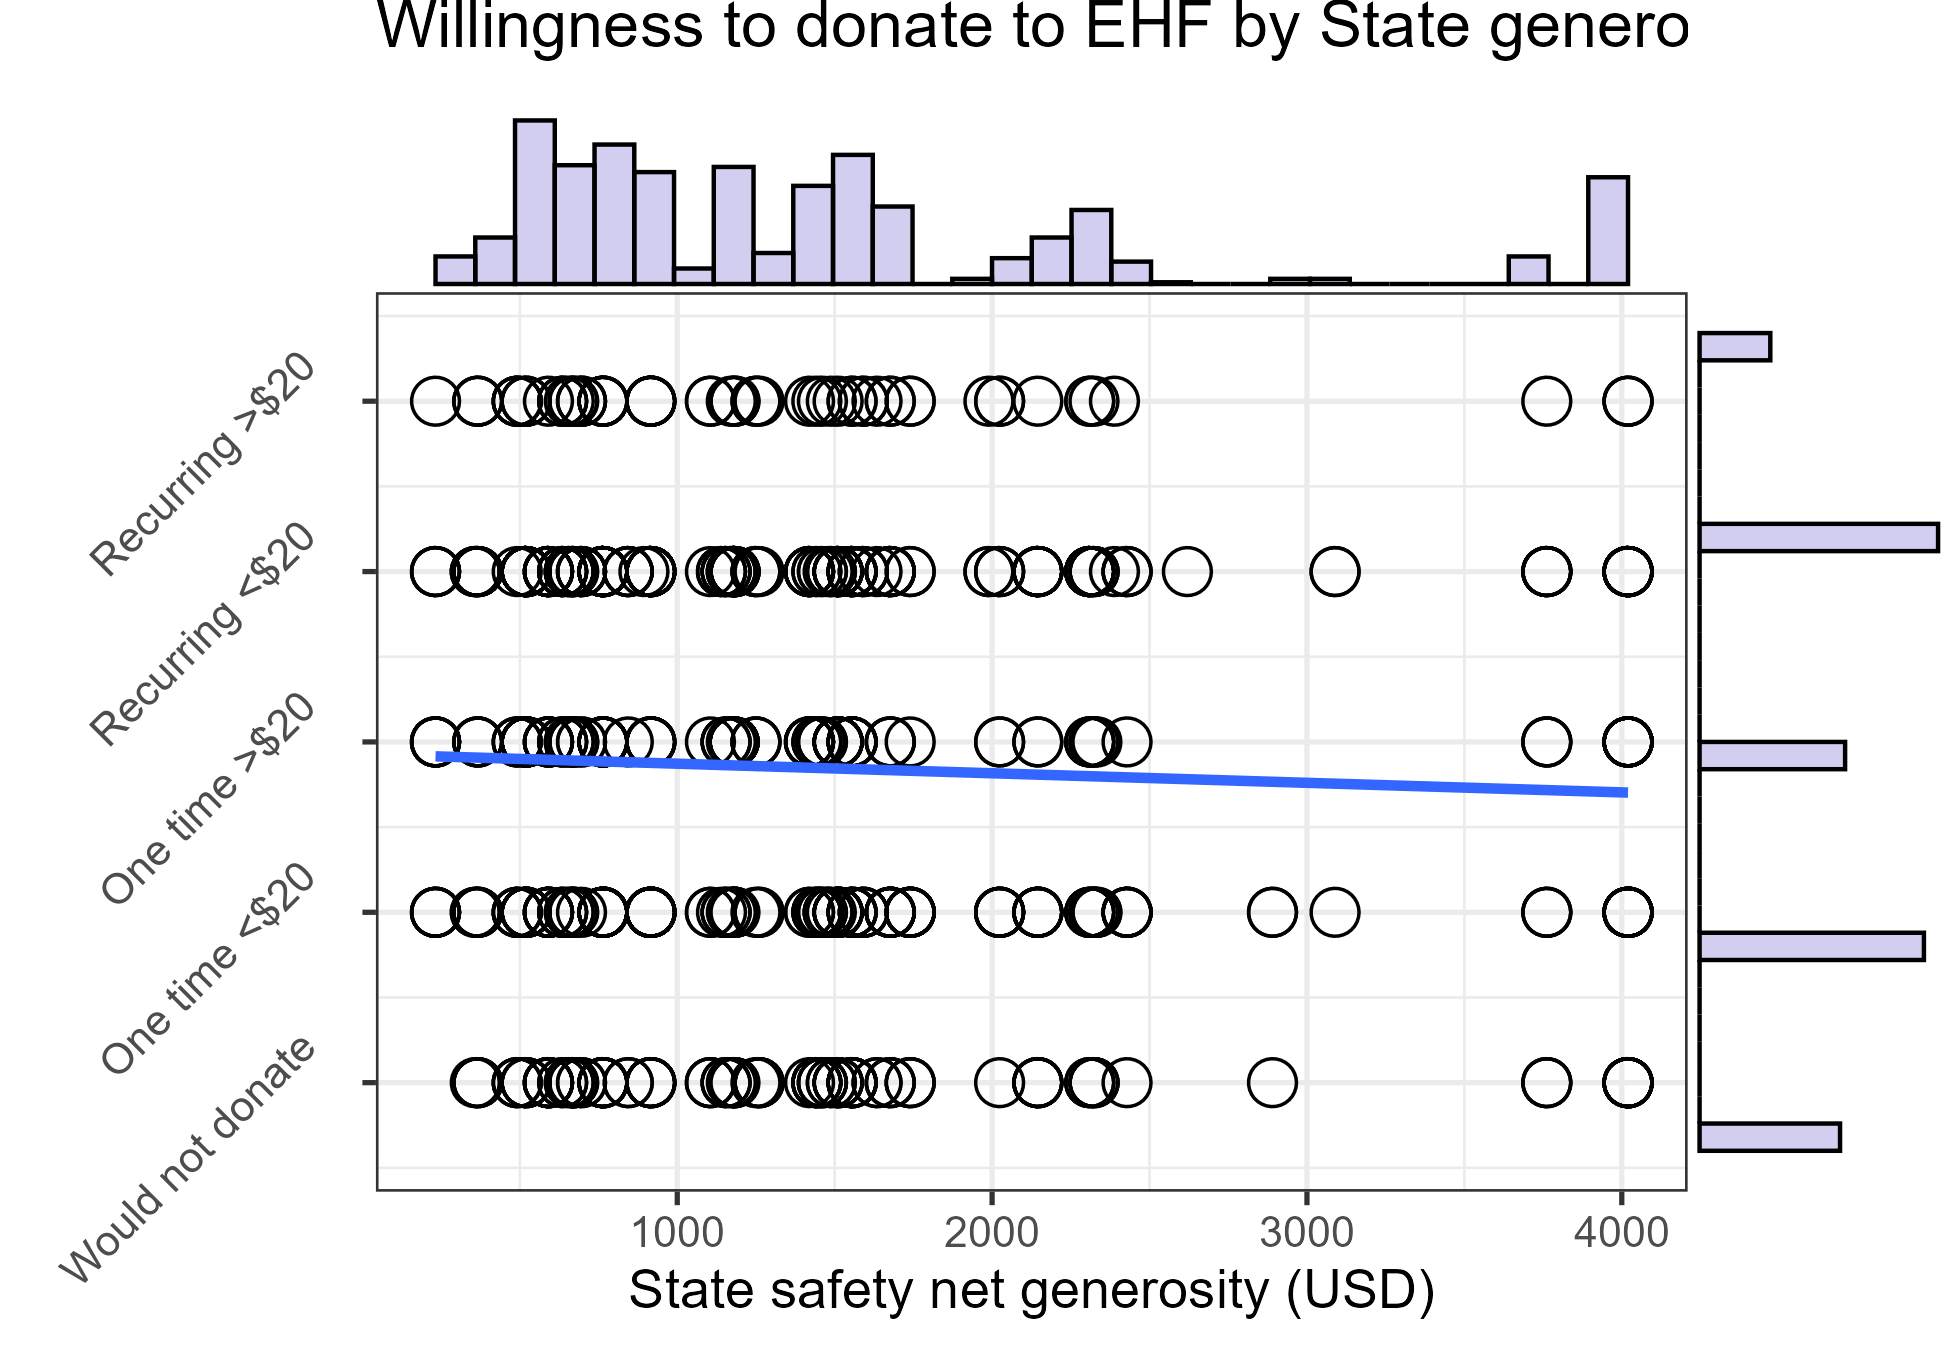
\includegraphics[width=0.5\linewidth]{../plots/ui_plot_gr_don} }

}

\caption{EHF support and willingness to donate to a potential new EHF, by state level welfare benefits in USD. Marginal distributions of the variables are included as blue histograms.}\label{fig:fig-ehf-genretail}
\end{figure}

We explore these relationships further using both linear regression and hierarchical linear models allowing for random intercepts as well as cross-state variation in the effect of political conservatism, both as a function of state-level safety net generosity. In addition to state safety net variables, we also include a variety of other covariates connected to charitable giving propensity and the substitution hypothesis. These include whether the respondent has used welfare in the past, religiosity, and whether the respondent identifies as politically conservative (\citeproc{ref-brooksWhoReallyCares2006}{Brooks 2006}; \citeproc{ref-bekkersWhoGivesLiterature2011}{Bekkers and Wiepking 2011b}; \citeproc{ref-wiepkingWhoGivesLiterature2012}{Wiepking and Bekkers 2012}; \citeproc{ref-andreoniCharitableGiving2013}{Andreoni and Payne 2013}).\footnote{Religiosity is a binary variable measuring if a respondent declared affiliation with any religion. Conservatism is also a binary variable, measuring whether the respondent placed themselves as ``Conservative'' or ``Leaning Conservative'' in a question about ideological identification.} Because appreciating real estate assets may depress support for the welfare state, we produce a measure of home value increases. Specifically, we multiply an indicator for home ownership with the 5-year change in the state-level home price index produced by the US Federal Housing Finance Agency. We include both terms of this product in Model E. We also condition on race, gender, age, education, and household income but do not report those for space considerations.

\begin{table}
\centering
\begin{talltblr}[         %% tabularray outer open
caption={Support for EHF among retail workers by state level safety net generosity models. There is no detected state level variation.  \label{tab:tab-genpop-ui-supp}},
note{}={* p \num{< 0.1}, ** p \num{< 0.05}, *** p \num{< 0.01}},
note{ }={Standard errors in parentheses. Additional covariates include age, gender, race, job tenure, hourly and full time status, college degree, whether the reported employment is their main job, income, religiosity.},
]                     %% tabularray outer close
{                     %% tabularray inner open
colspec={Q[]Q[]Q[]Q[]Q[]Q[]},
hline{2}={1-6}{solid, black, 0.05em},
hline{20}={1-6}{solid, black, 0.05em},
hline{1}={1-6}{solid, black, 0.08em},
hline{23}={1-6}{solid, black, 0.08em},
column{2-6}={}{halign=c},
column{1}={}{halign=l},
}                     %% tabularray inner close
& Model A & Model B & Model C & Model D & Model E \\
State safety net generosity & \num{-0.010} & \num{-0.012}* & \num{-0.013} & \num{-0.015} & \num{-0.009} \\
& (\num{0.007}) & (\num{0.007}) & (\num{0.010}) & (\num{0.011}) & (\num{0.010}) \\
Has an EHF & \num{0.023} & \num{0.023} & \num{0.022} & \num{0.023} & \num{0.023} \\
& (\num{0.020}) & (\num{0.021}) & (\num{0.023}) & (\num{0.023}) & (\num{0.023}) \\
Previous welfare recipient & \num{0.065}*** & \num{0.064}*** & \num{0.064}*** & \num{0.065}*** & \num{0.067}*** \\
& (\num{0.019}) & (\num{0.019}) & (\num{0.020}) & (\num{0.020}) & (\num{0.020}) \\
Conservative &  & \num{-0.014} & \num{-0.014} & \num{-0.029} & \num{-0.017} \\
&  & (\num{0.021}) & (\num{0.023}) & (\num{0.040}) & (\num{0.023}) \\
Generosity x Conservative &  &  &  & \num{0.010} &  \\
&  &  &  & (\num{0.023}) &  \\
Home owner &  &  &  &  & \num{-0.056} \\
&  &  &  &  & (\num{0.067}) \\
Home owner x house appreciation &  &  &  &  & \num{-0.000} \\
&  &  &  &  & (\num{0.001}) \\
Var: intercept &  &  & \num{0.019} & \num{0.018} & \num{0.271} \\
Var: house appreciation &  &  &  &  & \num{0.003} \\
Var: conservative &  &  &  & \num{0.004} &  \\
Var: residual &  &  & \num{0.277} & \num{0.278} & \num{0.275} \\
Model Type & Cluster-robust & Cluster-robust & HLM & HLM & HLM \\
$N$ & \num{1008} & \num{988} & \num{989} & \num{988} & \num{988} \\
AIC & 288 & 293 & 406 & 434 & 453 \\
\end{talltblr}
\end{table}\begin{table}
\centering
\begin{talltblr}[         %% tabularray outer open
caption={Willingness to donate to EHF among retail workers who do not have an EHF, by state level safety net generosity models. There is no detected state level variation. \label{tab:tab-genpop-ui-don}},
note{}={* p \num{< 0.1}, ** p \num{< 0.05}, *** p \num{< 0.01}},
note{ }={Standard errors in parentheses. Additional covariates include age, gender, race, job tenure, hourly and full time status, college degree, whether the reported employment is their main job, income, religiosity.},
]                     %% tabularray outer close
{                     %% tabularray inner open
colspec={Q[]Q[]Q[]Q[]Q[]Q[]},
hline{2}={1-6}{solid, black, 0.05em},
hline{18}={1-6}{solid, black, 0.05em},
hline{1}={1-6}{solid, black, 0.08em},
hline{21}={1-6}{solid, black, 0.08em},
column{2-6}={}{halign=c},
column{1}={}{halign=l},
}                     %% tabularray inner close
& Model A & Model B & Model C & Model D & Model E \\
State safety net generosity & \num{-0.011} & \num{-0.018}** & \num{-0.018} & \num{-0.014} & \num{-0.018} \\
& (\num{0.008}) & (\num{0.007}) & (\num{0.011}) & (\num{0.013}) & (\num{0.011}) \\
Previous welfare recipient & \num{0.060}*** & \num{0.061}*** & \num{0.061}** & \num{0.062}** & \num{0.061}** \\
& (\num{0.023}) & (\num{0.022}) & (\num{0.024}) & (\num{0.024}) & (\num{0.024}) \\
Conservative &  & \num{-0.021} & \num{-0.021} & \num{0.017} & \num{-0.023} \\
&  & (\num{0.033}) & (\num{0.029}) & (\num{0.060}) & (\num{0.029}) \\
Generosity x Conservative &  &  &  & \num{-0.029} &  \\
&  &  &  & (\num{0.035}) &  \\
Home owner &  &  &  &  & \num{0.033} \\
&  &  &  &  & (\num{0.081}) \\
Home owner x house appreciation &  &  &  &  & \num{-0.001} \\
&  &  &  &  & (\num{0.001}) \\
Var: intercept &  &  & \num{0.000} & \num{0.029} & \num{0.101} \\
Var: house appreciation &  &  &  &  & \num{0.001} \\
Var: conservative &  &  &  & \num{0.090} &  \\
Var: residual &  &  & \num{0.304} & \num{0.302} & \num{0.303} \\
Model Type & Cluster-robust & Cluster-robust & HLM & HLM & HLM \\
$N$ & \num{811} & \num{792} & \num{792} & \num{792} & \num{792} \\
AIC & 391 & 377 & 496 & 505 & 520 \\
\end{talltblr}
\end{table}

In Tables \ref{tab:tab-genpop-ui-supp} and \ref{tab:tab-genpop-ui-don} we present five models, of increasing complexity, that regress EHF support and willingness to donate to an EHF on state level generosity. The first two models are cluster robust standard error OLS models, with standard error clustering at the state level. Model A includes a suite of pre-registered covariates.\footnote{These are age, gender, race, college degree status, tenure at their job, whether this job is their primary job, and whether they work full-time. Ahlquist (\citeproc{ref-ahlquistPrivateWelfareCorporate2025}{2025}) shows that job tenure and full-time status are the primary predictors of pre-exposure to the EHF.} Model B additionally includes household income, whether the respondent identifies as politically conservative, religiosity, and home value appreciation calculated using the Federal Housing Finance Agency's House Price Index.

There is little evidence of correlation of state safety net generosity with support or willingness to donate to an EHF. Between the four estimated models, only Model B shows a statistically significant and negative effect (\(p<0.05\) for the donation outcome, \(p<0.1\) for the support outcome). This, in addition to the improving performance of Model B in terms of AIC, may indicate some omitted variable bias present in Model A that is accounted for by the inclusion of additional covariates in Model B.\footnote{This result is not driven by the slight decrease in sample size between Model A and the remaining four models. We run Model A on the support of Model B and find no difference in the reported results. Full regression tables for the limited models are omitted for parsimony.} There is, however, reason to question the importance of this finding in relation to our hypotheses. First, the magnitude of the point estimate is extremely small in comparison to the outcome variable, equal to approximately 0.05 of one standard deviation. It is also around a third of the effect of having previously received welfare. Second, this finding is not consistent with any other of the eight fitted models, and does not reach conventional levels of statistical significance for the EHF support outcome.

We then fit three additional hierarchical linear models (HLMs) which should be able to detect any state level variation either in the intercept or the slope of key variables, and compare that to the unexplained residual variance at the individual level. Large variances in the intercept term (relative to residual variance) indicate that, even after conditioning on all included variables, there is substantial unexplained variance at the state level. Large variance in the slope of the key variables would mean that the relationship between the key variable and the outcome is highly heterogeneous across states. If either of these are the case, then this could indicate some uncaptured variance at the state level that explains support for or willingness to donate to an EHF. That would be a potential threat to our conclusions, if the state-level variation is correlated with some unmeasured aspect of the state-level safety net.

All three models include the expanded set of covariates present in Model B. All models are estimated using restricted maximum likelihood methodology, which compensates for downward bias present in typical maximum likelihood estimation. Model C adds a random intercept term, which partially pools state-level intercept estimates. Model D adds a random slope estimate for the effect of identifying as a conservative on EHF support/willingness to donate, as well as a fixed-effect interaction term between generosity and conservative self-identification. Model E is similar to Model D, but replaces conservative identification with home price appreciation.

The majority of non-residual variances estimated by the HLMs are close to zero, which given the {[}0, 1{]} range of the response and the magnitude of the residual variance estimate, signify that no additional variance is explained by the hierarchical structure. The exception to this is the estimated state-level variance of the intercept term in Model E. However, a profile-likelihood confidence interval on the variance components of Model E shows the intercept variance is not distinguishable from zero (95\% CI: 0 -- 0.195 for donation, 0 - 0.261 for support) and the random slope on house price appreciation is negligible, with the correlation between them unidentifiable. This is consistent with a near-singular fit, rather than genuine state-level variation. When examining model performance, as our models become more complex, AIC values increase, indicating that the overall model fit is deteriorating, which would not be the case if the models were capturing substantial state-level variance.

The results, therefore, indicate little evidence in favor of either version of the substitution hypothesis. There is little to no variation in terms of state level effects on EHF support and willingness to donate that is explained through State-level variation in benefit generosity. Given this fact, and the findings of models B and D, we can also conclude that ideological identification as conservative also does not affect the correlation between State-level generosity and EHF support.

\section{Studies 2 \& 3}\label{sec-study2-3}

\subsection{Case selection}\label{case-selection}

Study 1 used a national sample and relied on respondent reports about their employer's EHF. Studies 2 and 3 zoom on two specific firms with well-established EHFs: Home Depot and Walmart. Both firms are large, national ``big box'' retailers that compete to some degree in product and labor markets. Both are large enough to make our independent recruitment of a survey sample feasible. They are matched on the features most likely to confound a comparison---industry, national scale, program vintage, and in-house EHF management---but they differ sharply in EHF generosity and promotion. This supports an extreme-case logic (\citeproc{ref-seawrightCaseSelectionTechniques2008}{\textbf{seawrightCaseSelectionTechniques2008?}}): Home Depot operates one of the oldest, most generous, and most heavily promoted EHFs. If a substitution effect exists, it should be easiest to detect among Home Depot workers. Walmart has a much smaller and lightly promoted EHF, which allows us to probe whether a modest EHF can move worker attitudes and lets us test whether program differences matter (H2b). With only two firms we cannot isolate \emph{which} differences drive any divergence, but we can establish whether EHF effects appear consistently across contexts. We briefly outline the two programs.

Home Depot has run the Homer Fund in-house since 1999. It is among the most generous EHFs: grants reach \$10,000 per qualifying event, eligibility begins on the first day of employment, and workers may apply repeatedly for new events. The program is substantial, disbursing \$21.2 million to more than 12,000 workers in fiscal 2022 (\citeproc{ref-thehomedepotEnvironmentalSocialGovernance2023}{Depot 2023}), the survey year. Home Depot also promotes the fund heavily through a dedicated website, a YouTube channel of professional testimonial videos, and active worker-facing social media. Home Depot regularly runs Homer Fund donation drives in which stores compete to generate donations.

Walmart's ACNT is likewise over two decades old and managed in-house, open to full- and part-time workers with at least 90 days' tenure. It is far less generous: grants are capped at \$1,500 across a rolling five-year window, regardless of how many qualifying events occur. Promotion appears minimal; there is little social-media presence and no evidence of donation drives comparable to Home Depot's.\footnote{Walmart does match employee donations to its political action committee \$2:1 with corporate donations to the Together Fund. Fewer than 1\% of our survey respondents reported contributing to the Walmart PAC.}

\subsection{The samples and surveys}\label{the-samples-and-surveys}

We follow Schneider and Harknett (\citeproc{ref-schneiderWhatFacebookTool2019}{2019}) and build matched worker--employer samples by recruiting respondents through targeted ads on Meta platforms (Facebook, Instagram, Threads), aimed at users 18 and older whom Meta identified as Home Depot or Walmart employees. Respondents who completed the survey were entered in a raffle for an iPad Mini or a Visa gift card. Schneider and Harknett (\citeproc{ref-schneiderWhatFacebookTool2019}{2019}) show that this approach generates samples that recover accurate estimates of firm-level workforce quantities in retail.\footnote{See also (\citeproc{ref-growFacebooksAdvertisingData2022}{\textbf{growFacebooksAdvertisingData2022?}})} Others have shown that this recruitment method performs well in similar contexts (\citeproc{ref-zhangQuotaSamplingUsing2020}{\textbf{zhangQuotaSamplingUsing2020?}}; \citeproc{ref-neundorfHowImproveRepresentativeness2023}{\textbf{neundorfHowImproveRepresentativeness2023?}}). Like any social-media recruitment strategy, there are concerns about selection bias. Because our quantities of interest are in-sample treatment effects (SATE) and we condition on the covariates on which we might construct weights, we do not apply survey weights in the experimental analysis. Targeted social media recruitment is currently the cost-effective method for generating large matched worker-employer samples in the US.

The Home Depot survey was fielded 7 September--15 October 2021, yielding 515 completed responses that passed an attention check and confirmed Home Depot employment. The Walmart survey ran 23 October--4 December 2024, producing 980 comparable responses. Summary statistics by treatment condition appear in Appendices \ref{app-survsum-uw} and \ref{app-wmt-survsum}.

The two surveys were closely matched in wording and ordering, with Study 3 adding several extensions, most importantly a behavioral donation measure (a click-through to a donation page at the end) and a placebo video condition in the experiment.

\subsection{EHF survey experiments}\label{ehf-survey-experiments}

In both studies 2 and 3, we randomly exposed respondents to messages about their employer's EHF to test H2, 2a, and 2b. The main quantities of interest are the average treatment effects (ATE) for each of the EHF treatments relative to control for each of the outcome variables; specifics on the treatments and outcomes of interest are presented in the following sections. For each, we present graphical displays as well as regression-based estimates.

Because we randomize \emph{information} rather than program access, some respondents arrive already aware of their employer's EHF. These ``pre-exposed'' workers may be less respondsive to the treatment than those learning of the program for the first time, so the ATE may understate the effect of informing a previously uninformed worker---a form of pre-exposure bias (\citeproc{ref-druckmanLearningMorePolitical2012a}{Druckman and Leeper 2012}; \citeproc{ref-ferrariMethodologicalApproachCausal2023}{Ferrari 2023}). We therefore examine treatment-effect heterogeneity by prior awareness.\footnote{We use ``aware'' and ``pre-exposed'' interchangeably.}

We measure prior awareness before treatment: respondents select, from a list of job amenities, those they believe they have access to. We code selection of ``emergency cash to help in times of need'' as EHF awareness.\footnote{(\citeproc{ref-ahlquistPrivateWelfareWorkplace2026}{\textbf{ahlquistPrivateWelfareWorkplace2026?}}) discusses this measure and compares it with alternative awareness measures. He also discusses the correlates of pre-exposure, the most important of which is job tenure.} When conditioning on pre-exposure, a causal interpretation of the treatment requires that pre-exposure be independent of potential outcomes conditional on treatment and pre-treatment covariates.\footnote{Equivalently, pre-exposure can be cast as treatment compliance---the pre-exposed as always-takers, the unaware as compliers---but because we measure pre-exposure directly, the heterogeneous-effects framing is more natural.}

In the analysis that follows, we report four models for each outcome. The first includes only the experimental treatment indicators, providing ATE estimates. The second adds a treatment-by-awareness interaction term. The third includes a suite of pre-registered pre-treatment covariates, as discussed above. The fourth, ``expanded'' model then adds additional covariates that were not pre-registered but that are relevant to the substitution hypothesis literatures: household income, whether the respondent identifies as politically conservative, religiosity, safety net generosity in the respondent's state of residence (\citeproc{ref-schmidtStateSafetyNet2024}{Schmidt, Shore-Sheppard, and Watson 2024}), and home value appreciation calculated using the Federal Housing Finance Agency's House Price Index. Following the pre-registered plan, we report linear regression models in the main text, employing robust or clustered standard errors, as appropriate

\subsubsection{Study 2}\label{study-2}

The experiment in Study 2 consisted of a control condition and two treatment arms, referred to as the \emph{text} and \emph{video} treatments, respectively. Respondents in the control arm saw no prompt or mention of the Home Depot EHF. Those in the text treatment saw a brief, neutral text description of the Homer Fund.\footnote{The wording of the text treatment was ``Your employer, The Home Depot, maintains a program called the Homer Fund. The Homer Fund combines donations from workers like you with money from the Home Depot corporation. The Homer Fund uses this money to offer cash grants of up to \$10,000 to Home Depot employees in times of unexpected financial hardship like a natural disaster, illness, or death in the family.''}

Neutral text descriptions do not reflect how employers actually communicate about these programs with their workers. Home Depot's YouTube channel hosts professional testimonial videos from purported grant recipients; respondents in the video arm watched the one shown in Figure \ref{fig:fig-ray}, panel (a), a 2:41 testimonial from ``Ray,'' a veteran and Home Depot worker whose family received Homer Fund support during a serious illness.\footnote{The video is available at \url{https://www.youtube.com/watch?v=qF-HBoySMe}.}

Our key outcomes of interest in Study 2 comes from a battery of questions asking respondents to report how much responsibility the government should have for ensuring the welfare of different groups, with responses in four categories ranging from ``none at all'' to ``a lot''. Here we examine responses for ``the unemployed''. This question format, taken from the General Social Survey, is also part of the ISSP ``role of government'' module and is widely used for gauging attitudes toward government social insurance and welfare activities (\citeproc{ref-blekesaunePublicAttitudesWelfare2003}{Blekesaune and Quadagno 2003}; \citeproc{ref-beanComparisonMassAttitudes1998}{Bean and Papadakis 1998}; \citeproc{ref-rehmInsecureAlliancesRisk2012}{Rehm, Hacker, and Schlesinger 2012}; \citeproc{ref-deemingPoliticsFracturedSolidarity2018}{Deeming 2018}). We will interpret responses to this question as reflecting support for government-provided unemployment insurance (UI).

\begin{figure}

{\centering \subfloat[Home Depot\label{fig:fig-ray-1}]{\includegraphics[width=0.5\linewidth]{../plots/RaysStory} }\subfloat[Walmart\label{fig:fig-ray-2}]{
\includegraphics[width=0.5\linewidth]{../plots/Rays_story_wmt} }

}

\caption{Screen stills of the video treatments}\label{fig:fig-ray}
\end{figure}

\paragraph{Attitudes toward social insurance}\label{attitudes-toward-social-insurance}

The left panel of Figure \ref{fig:fig-ui} displays the distribution of responses by EHF treatment status for Study 2. Overall, workers in the Home Depot sample are quite favorable toward government support for the unemployed, with a solid majority viewing the government as at least somewhat responsible for the welfare of the unemployed. The video treatment clearly \emph{reduces} the proportion of responses in the ``none'' category in favor of the two positive categories. In other words, treatment made respondents \emph{more} rather than less supportive of government-provided social insurance, contrary to the substitution hypothesis. The text treatment, on the other hand, does not appear to have any detectable treatment effect on average.

\begin{figure}

{\centering \subfloat[Study 2\label{fig:fig-ui-1}]{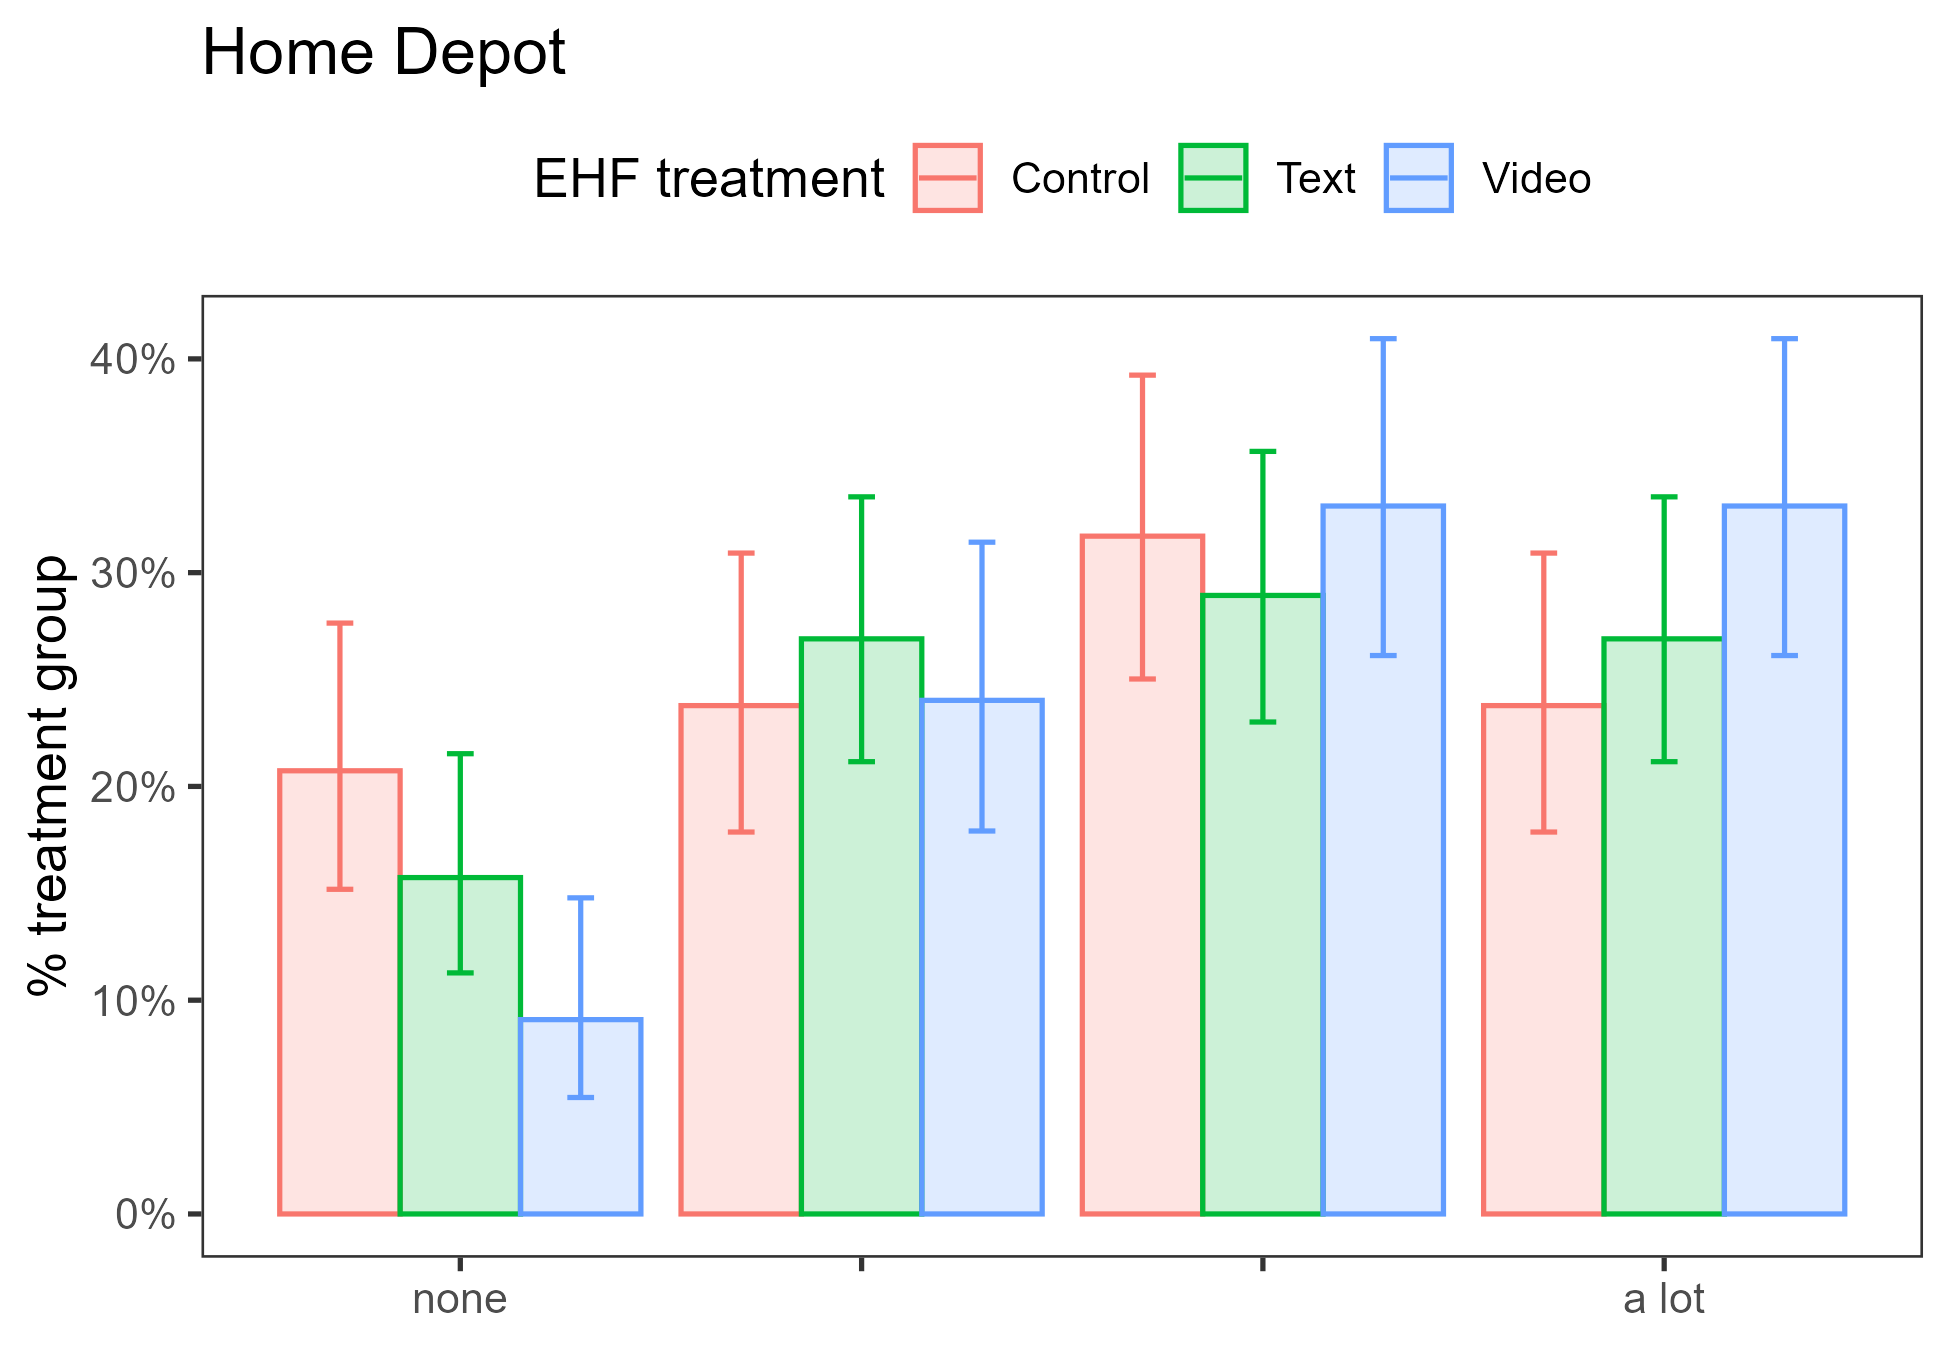
\includegraphics[width=0.5\linewidth]{../plots/ui_plot_thd} }\subfloat[Study 3\label{fig:fig-ui-2}]{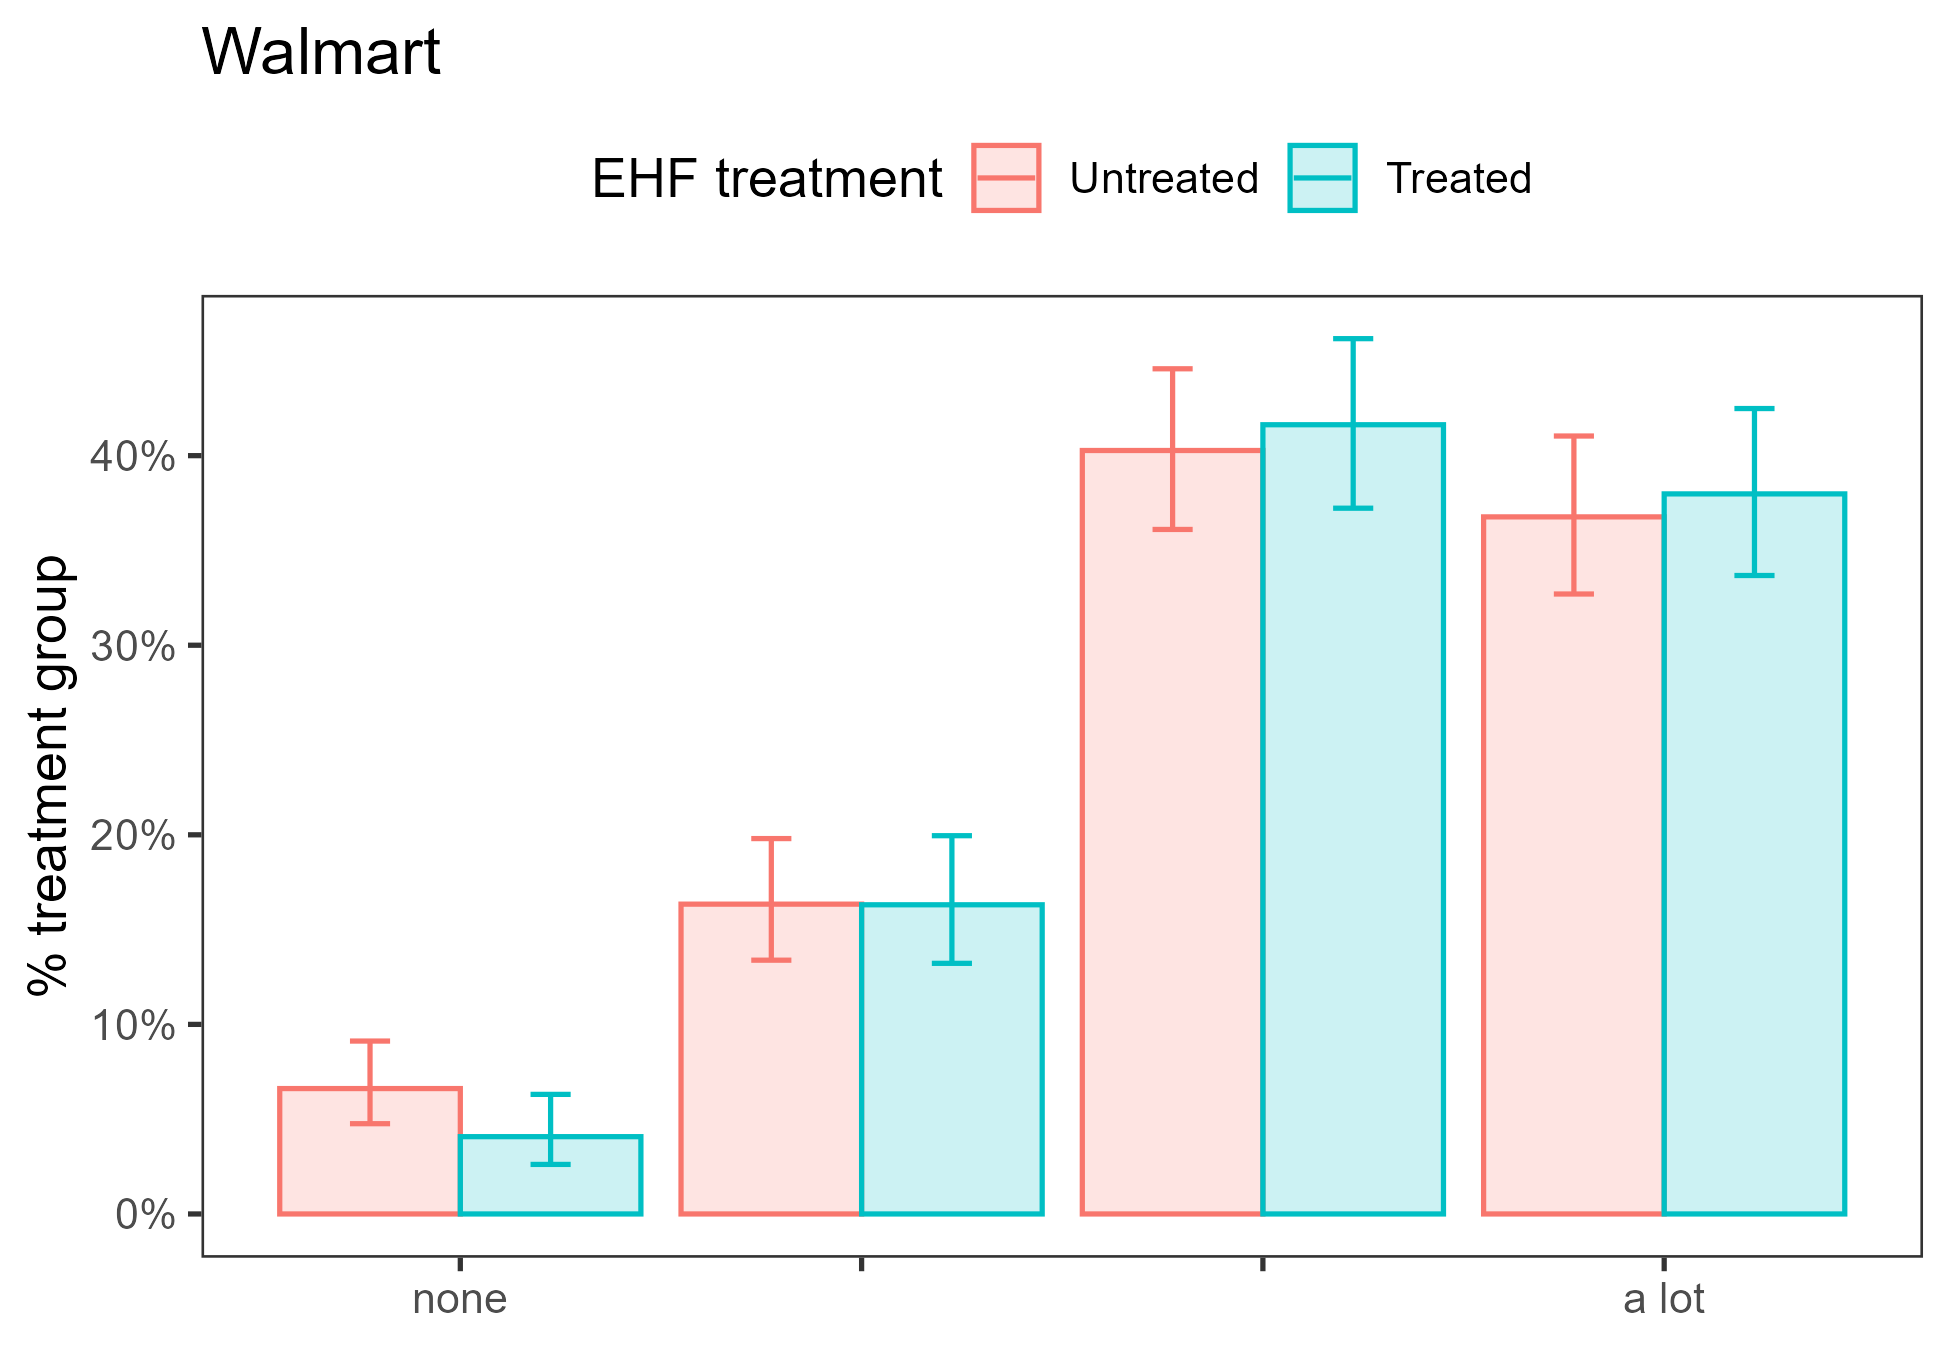
\includegraphics[width=0.5\linewidth]{../plots/ui_plot_wmt} }

}

\caption{Government responsibility for supporting the unemployed, by EHF treatment status.  Vertical bars are 95\% confidence intervals.}\label{fig:fig-ui}
\end{figure}

In Table \ref{tab:tab-ui}, we display estimates from a series of linear regression models on UI support. The first model, including only experimental treatments, confirms a positive average treatment effect for the video treatment of about 0.31 standard deviations. Looking at the second model that accounts for pre-exposure, we find that respondents pre-exposed to the Home Depot EHF are -0.3 standard deviations less supportive of UI than the unaware (\(p<0.1\)), but we find no treatment effects among the unaware. Contrary to the substitution hypothesis, we do find positive treatment effects among the \emph{pre-exposed}, especially for the video treatment. Adding pre-registered covariates, including those that predict EHF pre-exposure (the third model), does not meaningfully alter interpretation. The final model in Table \ref{tab:tab-ui} includes a whole series of predictors connected to the substitution hypothesis, entered as linear terms.\footnote{There was no evidence that the the treatment effect was moderated by state-level welfare generosity or respondent conservativeness.} More conservative respondents are less supportive of government support for the unemployed. Income, past use of welfare benefits, religiosity, and increased home values are all unrelated to support for UI conditional on treatment. Those living in states with more generous public safety nets are more positive about government support for the unemployed, even after conditioning on conservativeness, which may reflect some geographic sorting.

\begin{table}
\centering
\begin{talltblr}[         %% tabularray outer open
caption={Government support for the unemployed (Home Depot) \label{tab:tab-ui}},
note{}={* p \num{< 0.1}, ** p \num{< 0.05}, *** p \num{< 0.01}},
note{ }={Standard errors in parentheses.
 Pre-registered covariates include age, gender race, job tenure, hourly status, full time status, college degree, and main job.},
]                     %% tabularray outer close
{                     %% tabularray inner open
colspec={Q[]Q[]Q[]Q[]Q[]},
hline{2}={1-5}{solid, black, 0.05em},
hline{24}={1-5}{solid, black, 0.05em},
hline{1}={1-5}{solid, black, 0.08em},
hline{28}={1-5}{solid, black, 0.08em},
column{2-5}={}{halign=c},
column{1}={}{halign=l},
}                     %% tabularray inner close
& Base & Pre-exposure & Pre-registered & Expanded \\
Text treatment & \num{0.032} & \num{-0.053} & \num{-0.057} & \num{-0.073} \\
& (\num{0.037}) & (\num{0.062}) & (\num{0.062}) & (\num{0.055}) \\
Video treatment & \num{0.108}*** & \num{0.031} & \num{0.032} & \num{-0.009} \\
& (\num{0.038}) & (\num{0.060}) & (\num{0.059}) & (\num{0.059}) \\
Pre-exposed &  & \num{-0.105}* & \num{-0.102}* & \num{-0.090}** \\
&  & (\num{0.057}) & (\num{0.055}) & (\num{0.044}) \\
Text x pre-exposed &  & \num{0.141}* & \num{0.148}* & \num{0.142}* \\
&  & (\num{0.078}) & (\num{0.076}) & (\num{0.080}) \\
Video x pre-exposed &  & \num{0.127} & \num{0.116} & \num{0.117}* \\
&  & (\num{0.078}) & (\num{0.076}) & (\num{0.067}) \\
Past welfare &  &  &  & \num{0.010} \\
&  &  &  & (\num{0.043}) \\
HH income &  &  &  & \num{-0.000} \\
&  &  &  & (\num{0.001}) \\
Religiosity &  &  &  & \num{-0.021} \\
&  &  &  & (\num{0.035}) \\
State safety net generosity &  &  &  & \num{0.020}** \\
&  &  &  & (\num{0.009}) \\
Conservative &  &  &  & \num{-0.213}*** \\
&  &  &  & (\num{0.042}) \\
House appreciation &  &  &  & \num{-0.001} \\
&  &  &  & (\num{0.001}) \\
$N$ & \num{511} & \num{511} & \num{506} & \num{437} \\
Std. Errors & robust & robust & robust & state-clustered \\
$R^2$ & \num{0.02} & \num{0.02} & \num{0.09} & \num{0.17} \\
AIC & \num{362.4} & \num{364.0} & \num{340.1} & \num{273.7} \\
\end{talltblr}
\end{table}

To interpret the heterogeneous treatment effects more easily, Figure \ref{fig:fig-uieff} displays treatment effects by respondent pre-exposure to the EHF, derived from the second model. In the case of support for the unemployed, we see that treatment effects are entirely concentrated among those \emph{already} aware of the Home Depot's EHF. Contrary to expectations, both the text and video treatments \emph{increase} support for UI, although only the latter crosses conventional significance thresholds.

\begin{figure}
\centering
\pandocbounded{
\includegraphics[keepaspectratio]{Ahlquist_Ntounias_EHF_SI_2026_files/Ahlquist_Ntounias_EHF_SI_2026_files/figure-latex/fig-uieff-1.pdf}}
\caption{\label{fig:fig-uieff}Interpreting treatment effects on support for government aid to unemployed}
\end{figure}

Is unemployment support the appropriate policy to link with the EHF? After all, the EHF is designed to provide benefits to workers at a particular firm, whereas UI is a cushion in the event of job loss.\footnote{The pre-exposed may better appreciate this distinction, which may help explain the unexpected findings.} Two pieces of evidence suggest that UI is a reasonable policy domain to link with EHFs. First, although a Home Depot worker who loses her job can no longer apply for EHF support, workers are eligible for EHF grants if an immediate family member loses their job. Second, the UI question was asked as part of a battery of questions asking about two other policy areas: government support for the elderly and the provision of childcare for working parents. These two questions can constitute ``placebos'' since EHFs have no connection with either policy area. Parameter estimates from regressing support for these alternative policy areas on the EHF treatments and EHF awareness appear in Appendix \ref{app-placebo}. There is no evidence for any relationship between the EHF treatments and support for government involvement in either elder support or childcare, regardless of whether the respondent was aware of the EHF going into the survey and adjusting for predictors of awareness as well as predictors relevant to the substitution hypothesis.

In sum: Study 2 provides no evidence consistent with the substitution hypothesis. Pre-exposed respondents reacted to treatment differently than the unexposed, but the effects observed were in the opposite the expected direction under H2. We see no evidence consistent with the hypothesis that employer-provided ``private welfare'' crowds out support for the social safety net. If anything, the EHF treatment increases support for government action to support the unemployed.

\subsubsection{Study 3}\label{study-3}

Study 3's experiment parallels Study 2, with awareness of the ACNT measured using the same question format. But study 3 includes three changes. First, because the text arm performed weakly at Home Depot, we used only a video treatment for Walmart. Unfortunately Walmart produces analog to the Home Depot's testimonials, so we created our own. Using the Homer Fund video as script and audiovisual template, we hired a paid actor and adapted the video to the Walmart context; Figure \ref{fig:fig-ray}, panel (b) shows an opening still.\footnote{The actor matched the Homer Fund spokesperson's gender (male) and race (white) and was judged to be of similar age by mTurk coders. The Walmart video ran 41 seconds shorter, achieved by trimming interstitial and panning shots and Home-Depot-specific passages rather than substantive script. Appendix \ref{app-vidsim} provides multimodal (visual, acoustic, and semantic) similarity evidence that the two treatment videos are close analogs and that the placebo shares their audiovisual form but not their content.}

Second, to distinguish the effect of EHF messaging from a generic ``video effect,'' Study 3 adds a placebo arm in which the same actor reads a Walmart press release about its Vizio acquisition.\footnote{Videos: \href{https://tinyurl.com/EHF-Study3-placebo}{placebo}; \href{https://tinyurl.com/EHFStudy3-solidarity}{treatment, solidarity card}; \href{https://tinyurl.com/EHF-Study3-charity}{treatment, charity card}.} Respondents were assigned to treatment or control with equal probability, and controls were split between a pure control (no information, as in Study 2) and the placebo.\footnote{We also pre-registered a sub-experiment varying the still ``card'' shown before the video plays: a \emph{solidarity} framing emphasizing support for fellow Walmart workers versus a \emph{charity} framing emphasizing donations to those in need. The video was otherwise identical across arms. We found no detectable difference between framings and so do not discuss it in the main text; see Appendix \ref{app-framing}.} Manipulation checks (Appendix \ref{app-wmt-manip}) confirm the video raised ACNT awareness while the placebo did not, so we report binary treatment/control below.

Third, we modified the outcomes we study in two ways. In the Walmart survey we again used the GSS question battery and asked respondents about the level of government responsibility for ensuring the living standards of the unemployed. But to more closely link outcome measurement with EHFs, we substituted a question asking about government responsibility for ``people confronting short-term hardships'' for the childcare question in Study 2. We also created a behavioral indicator of donation willingness to the Walmart EHF. At the end of Study 3, respondents had the opportunity to click on a link to take them to a page where they could donate to the ACNT. Based on past research, we expect those exposed to the emotional appeal in the video to be more willing to donate (\citeproc{ref-andreoniPowerAskingHow2011}{Andreoni and Rao 2011}; \citeproc{ref-bekkersLiteratureReviewEmpirical2011}{Bekkers and Wiepking 2011a}). We examine whether the generosity of the state safety net moderates this treatment effect.

\paragraph{Attitudes toward social insurance and emergency government aid}\label{attitudes-toward-social-insurance-and-emergency-government-aid}

The right panel of Figure \ref{fig:fig-ui} displays the Study 3 response distribution for the unemployment support outcome while the left panel of Figure \ref{fig:fig-emerg-donate} displays the response distribution for the emergency aid outcome. Over 80\% of the Walmart sample agreed that the government should take at least some responsibility for the living standards of the unemployed, a much higher rate than among the Home Depot workers. The Walmart sample exhibited a similar level of support for government aid to those facing hardship. Among the Walmart sample, there is no treatment effect apparent for either outcome. Although the pattern of responses for UI for Walmart is similar to Study 2: those in the treatment group were less likely to say that the government has no responsibility for the unemployed, contrary to the substitution hypothesis.

\begin{figure}

{\centering \subfloat[emergency aid\label{fig:fig-emerg-donate-1}]{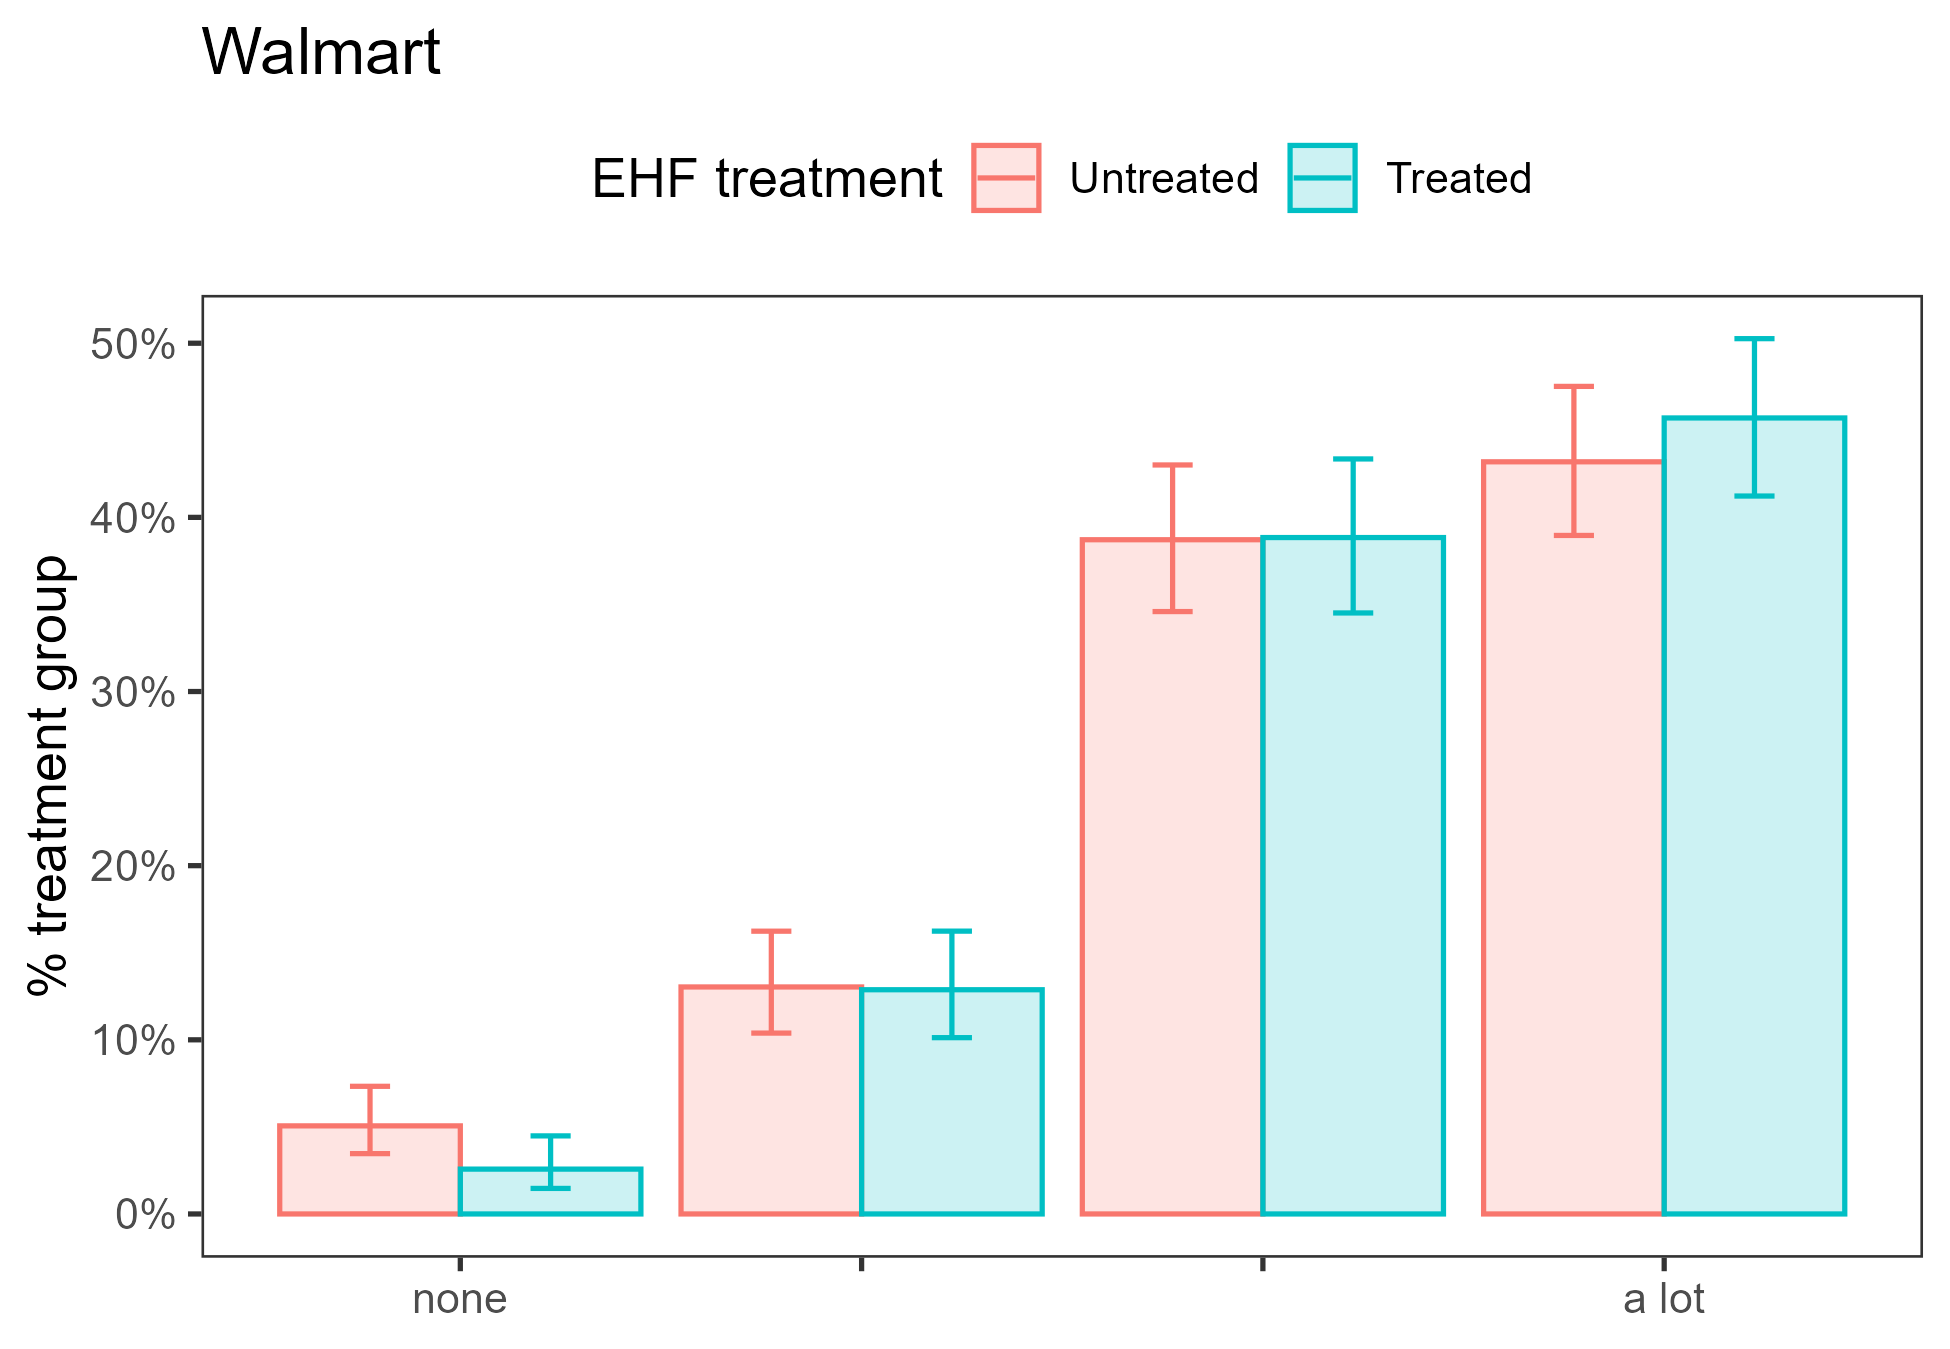
\includegraphics[width=0.5\linewidth]{../plots/emerg_plot_wmt} }\subfloat[ACNT donation\label{fig:fig-emerg-donate-2}]{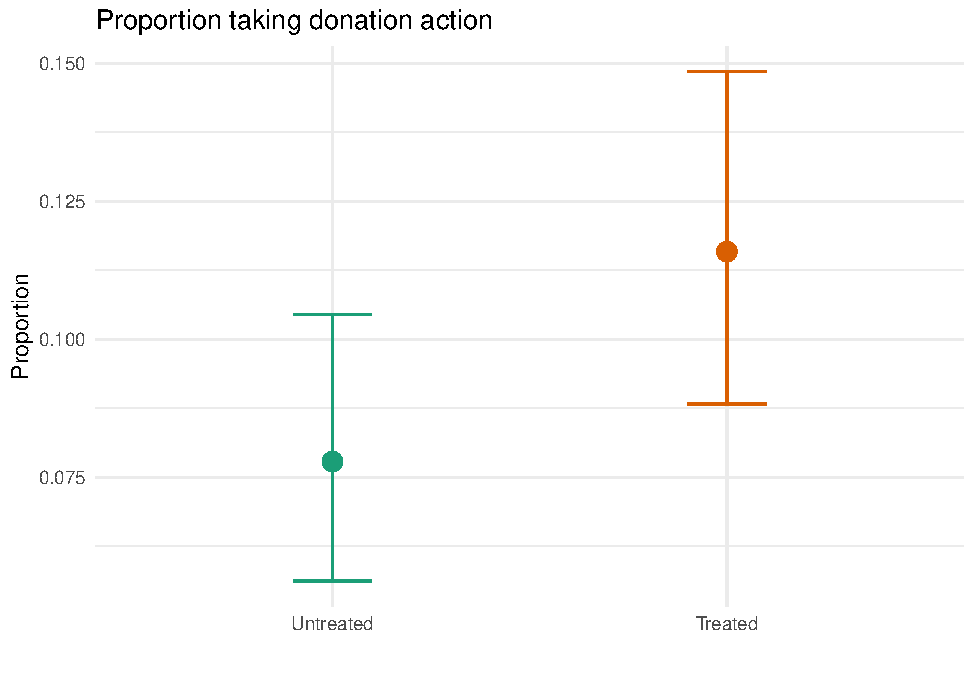
\includegraphics[width=0.5\linewidth]{../plots/donate_wmt} }

}

\caption{Additional Walmart outcomes, by EHF treatment status.  Vertical bars are 95\% confidence intervals.}\label{fig:fig-emerg-donate}
\end{figure}

Table \ref{tab:tab-ui-hard-wmt} displays regression results that reinforce the null relationship in Figures \ref{fig:fig-ui} and \ref{fig:fig-emerg-donate}. There is no evidence of a treatment effect for either outcome. Pre-exposure to the ACNT and additional covariates make no difference in this conclusion. In the ``expanded'' model we continue to see that conservatives are less supportive of government activity to support the unemployed and those facing temporary hardship. Walmart workers who have seen their home values appreciate are less supportive of UI but there is no relationship between home appreciation and support for government aid to those facing temporary hardship. More religious respondents are significantly less supportive of aid to those in temporary need. The generosity of the State-level safety net has no connection to respondents attitudes for either outcome.

\begin{table}[!h]
\centering\centering
\caption{\label{tab:tab-ui-hard-wmt}Support for unemployment insurance and emergency government aid (Walmart) \label{tab:tab-ui-hard-wmt}}
\centering
\resizebox{\textwidth}{!}{\begin{threeparttable}
\fontsize{7}{9}\selectfont
\begin{tabular}[t]{lccc>{}c|cccc}
\toprule
\multicolumn{1}{c}{ } & \multicolumn{4}{c}{DV: Unemployed} & \multicolumn{4}{c}{DV: Emergency} \\
\cmidrule(l{3pt}r{3pt}){2-5} \cmidrule(l{3pt}r{3pt}){6-9}
  & Base & Pre-exposed & Pre-registered & Expanded & Base  & Pre-exposed  & Pre-registered  & Expanded \\
\midrule
Treated & \num{0.016} & \num{0.018} & \num{0.016} & \num{0.007} & \num{0.019} & \num{0.012} & \num{0.012} & \num{-0.002}\\
 & (\num{0.014}) & (\num{0.017}) & (\num{0.018}) & (\num{0.016}) & (\num{0.013}) & (\num{0.017}) & (\num{0.017}) & (\num{0.015})\\
Pre-exposed &  & \num{0.003} & \num{0.007} & \num{-0.001} &  & \num{-0.007} & \num{-0.005} & \num{-0.015}\\
 &  & (\num{0.020}) & (\num{0.020}) & (\num{0.014}) &  & (\num{0.019}) & (\num{0.020}) & (\num{0.020})\\
Treated x pre-exposed &  & \num{-0.005} & \num{-0.005} & \num{0.006} &  & \num{0.017} & \num{0.014} & \num{0.026}\\
 &  & (\num{0.028}) & (\num{0.028}) & (\num{0.028}) &  & (\num{0.027}) & (\num{0.027}) & (\num{0.025})\\
Past welfare &  &  &  & \num{0.013} &  &  &  & \num{0.016}\\
 &  &  &  & (\num{0.016}) &  &  &  & (\num{0.017})\\
HH income &  &  &  & \num{-0.000} &  &  &  & \num{-0.000}\\
 &  &  &  & (\num{0.000}) &  &  &  & \vphantom{1} (\num{0.000})\\
Religiosity &  &  &  & \num{0.003} &  &  &  & \num{-0.017}\\
 &  &  &  & (\num{0.013}) &  &  &  & (\num{0.011})\\
State safety net generosity &  &  &  & \num{-0.008} &  &  &  & \num{-0.004}\\
 &  &  &  & (\num{0.006}) &  &  &  & (\num{0.007})\\
Conservative &  &  &  & \num{-0.061}*** &  &  &  & \num{-0.057}***\\
 &  &  &  & (\num{0.017}) &  &  &  & (\num{0.020})\\
House appreciation &  &  &  & \num{-0.000}*** &  &  &  & \num{-0.000}\\
 &  &  &  & (\num{0.000}) &  &  &  & (\num{0.000})\\
\midrule
Std Errors & robust & robust & robust & state-clustered & robust & robust & robust & state-clustered\\
$N$ & \num{980} & \num{980} & \num{980} & \num{913} & \num{980} & \num{980} & \num{980} & \num{913}\\
$R^2$ & \num{0.00} & \num{0.00} & \num{0.01} & \num{0.05} & \num{0.00} & \num{0.00} & \num{0.01} & \num{0.04}\\
AIC & \num{-222.9} & \num{-219.0} & \num{-216.2} & \num{-209.3} & \num{-320.9} & \num{-317.3} & \num{-313.4} & \num{-299.2}\\
\bottomrule
\end{tabular}
\begin{tablenotes}
\footnotesize
\item * p $<$ 0.1, ** p $<$ 0.05, *** p $<$ 0.01 Standard errors in parentheses. Pre-registered covariates include age, gender, race, job tenure, hourly status, full-time status, college degree, and main job. Both DV panels report identical specifications.
\end{tablenotes}
\end{threeparttable}}
\end{table}

Walmart has a substantially less generous EHF than the Home Depot. Given the findings in Studies 1 and 2, the null findings in Study 3 are unsurprising. Exposing Walmart workers to videos about their employers' EHF had no effect on their attitudes toward unemployment benefits or government emergency aid, although Walmart workers were, overall, much more supportive of these programs.

\paragraph{Willingness to donate to the Walmart EHF}\label{willingness-to-donate-to-the-walmart-ehf}

Study 3 included an opportunity to click a link to donate to the ACNT. As the right panel in Figure \ref{fig:fig-emerg-donate} shows, there is a low baseline willingness to take this action of 8\% in the Walmart sample. Nevertheless, those seeing the EHF video were about 4 percentage points (or 35\%, \(p < 0.05\)) more likely to take an action to donate.

\begin{table}[!h]
\centering\centering
\caption{\label{tab:fig-emerg-donate}ACNT donation willingness (Walmart sample) \label{tab:tab-donate-wmt}}
\centering
\resizebox{\textwidth}{!}{\begin{threeparttable}
\fontsize{8}{10}\selectfont
\begin{tabular}[t]{lccccc}
\toprule
  & Base & State Generosity & Pre-exposure & Pre-registered & Expanded\\
\midrule
Treated & \num{0.038}** & \num{0.075}** & \num{0.031} & \num{0.033} & \num{0.027}\\
 & (\num{0.019}) & (\num{0.036}) & (\num{0.025}) & (\num{0.025}) & (\num{0.030})\\
Pre-exposed &  &  & \num{-0.021} & \num{-0.017} & \num{-0.024}\\
 &  &  & (\num{0.024}) & (\num{0.024}) & (\num{0.021})\\
Treated x pre-exposed &  &  & \num{0.017} & \num{0.011} & \num{0.019}\\
 &  &  & (\num{0.039}) & (\num{0.038}) & (\num{0.045})\\
State safety net generosity &  & \num{0.011} &  &  & \num{-0.006}\\
 &  & (\num{0.013}) &  &  & (\num{0.011})\\
Treated x generosity &  & \num{-0.029} &  &  & \\
 &  & (\num{0.023}) &  &  & \\
Past welfare &  &  &  &  & \num{-0.005}\\
 &  &  &  &  & \vphantom{1} (\num{0.022})\\
HH income &  &  &  &  & \num{0.000}\\
 &  &  &  &  & \vphantom{1} (\num{0.000})\\
Religiosity &  &  &  &  & \num{0.037}*\\
 &  &  &  &  & (\num{0.022})\\
Conservative &  &  &  &  & \num{-0.039}*\\
 &  &  &  &  & (\num{0.021})\\
House appreciation &  &  &  &  & \num{-0.000}\\
 &  &  &  &  & (\num{0.000})\\
\midrule
Std Errors & robust & state-clustered & robust & robust & state-clustered\\
N & \num{980} & \num{980} & \num{980} & \num{980} & \num{913}\\
AIC & \num{386.8} & \num{388.9} & \num{390.2} & \num{389.6} & \num{409.9}\\
\bottomrule
\end{tabular}
\begin{tablenotes}
\small
\item * p $<$ 0.1, ** p $<$ 0.05, *** p $<$ 0.01 Standard errors in parentheses.
 Pre-registerd covariates include age, gender race, job tenure, hourly status, full time status, college degree, and main job.
\end{tablenotes}
\end{threeparttable}}
\end{table}

Table \ref{tab:tab-donate-wmt} presents regression-based estimates of treatment effects, using linear probability models.\footnote{See \ref{app-wmt-altdonate} for estimates using logistic regression and Firth regression to address concerns with rare events. Estimated treatment effects are quite similar across models.} Treatment significantly increases willingness to take an action to donate. There is no evidence that either state-level generosity or ACNT pre-exposure moderates these treatment effects.\footnote{Hierarchical logit models including state-level random effects and random slopes produce the same conclusion.} The inclusion of additional covariates does nothing to alter these conclusions.

The ACNT treatment did significantly increase willingness to donate, as expected, indicating that the treatment did work. But there is no evidence to support the claim that welfare generosity has any effect on the willingness of workers to donate to an EHF program. Across all three studies, we see no evidence consistent with either H1 or H2.

\subsection{Threats to Inference and Interpretation}\label{threats-to-inference-and-interpretation}

Null effects like those we just presented are notoriously difficult to defend. We briefly consider three inferential threats: that the experiments simply failed, that they were underpowered, and that workers are indifferent or antagonistic to EHFs. None survives scrutiny.

The experiments were not broken. Manipulation checks confirm that our treatments did what they were designed to do: exposure significantly raised awareness of the employer's EHF, while the Study 3 placebo moved awareness not at all.

Nor are the null results an artifact of insufficient power. In study 2, the experiment reliably detects treatment effects of about 0.11 on the 0--1 outcome scale (a minimum detectable effect of 0.107 at 80\% power), roughly a third of a standard deviation. The experiment did detect effects of that magnitude, only in the \emph{wrong direction} relative to the substitution hypothesis. In Study 3, the experiment can detect even smaller effects thanks to its larger sample size; the minimum detectable effect for the UI question falls to about 0.04 scale points or 0.17 standard deviations. Thus the research design is capable of ruling out an effect large enough to bear on the substitution hypothesis.

Finally, the nulls do not reflect workers disliking or dismissing EHF programs. Evidence points the other way. The companion paper shows that retail workers view EHFs favorably once they learn of them and EHF messaging can meaningfully increase attachment to the employer and dampen support for unionization. Workers do respond to EHF messages expressing approval, feeling more bound to their firm, and, when asked, donating at higher rates. What they do not do is revise their views about government responsibility for social insurance in response to a private program. The nulls we report are therefore a substantive finding: EHFs can move workers' orientation toward their employer without displacing their expectations of government.

\section{Discussion and Conclusion}\label{sec-conclusion}

There is a significant scholarly tradition arguing about whether private resources and charitable activities are substitutes for public welfare and social insurance. These literatures have virtually ignored the workplace, even though employers have tremendous flexibility to introduce or modify benefit plans and workplace programs that address a variety of economic risks. EHFs are one such tax-incentivized program that has received virtually no systematic study. This oversight is all the more remarkable as EHFs clearly echo both an earlier era of welfare capitalism and past mutual aid initiatives. Do these programs influence workers' attitudes and behaviors in ways consistent with the ``substitution hypothesis''?

Based on three pre-registered studies, our answer is a definitive ``no.'' In Study 1, we found little evidence that state-level welfare effort predicts support for or donation willingness to EHFs. In Studies 2 and 3, using survey experiments, there was no evidence that EHFs reduce support for government unemployment benefits or emergency aid, regardless of the substantial differences in generosity across the Home Depot and Walmart programs. In the Home Depot sample, the treatment induced a modest but significant \emph{increase} in support for government-provided UI among workers already aware of the EHF. This may be because these workers having a better understanding of the limitations of the EHF program. In Study 3, the treatment effect on EHF donations did not vary by state welfare generosity, contrary to expectations. Findings in these surveys are inconsistent with a simple ``private options crowd out public benefits'' story.

Our studies are not designed to speak to these mechanisms, but findings do point toward future research. The lack of any substitution effect between EHFs and support for public assistance suggests that EHFs may represent a reconfiguration of the moral economy of low-wage work. Strong worker interest in EHFs may reflect pessimism about the fraying safety net in the US. Rather than a substitute for social insurance and assistance, EHFs may be low-cost signals of corporate values and selective benevolence. Direct comparison between attitudes toward government- and employer-provided benefits would be instructive here.

An alternative interpretation is that EHFs are simply too new, too uncertain, or too small to matter yet. More probing, perhaps through interviews or analysis of online worker forums could shed light here. EHFs also emerged in the US, where the social safety net is particularly weak, inequality is stark, and regional variation in economic prospects continue to diverge. Cross national research in worker interest in EHF-type programs might speak to interesting variation in this regard.

Finally, political scientists have paid limited attention to how knowledge of government programs affects private charitable behavior, despite theoretical reasons to expect that information constraints may moderate crowding out effects. This represents an important avenue for future research, particularly relevant to understanding how employee knowledge of government programs might affect workplace charity.

From a policy perspective, EHFs appear to answer a felt need among low-wage retail workers. They operate in the shadow of eroded public welfare institutions, yet draw part of their funding from favorable tax treatment, a private, partial complement to a slow public system. Employer-proved aid can have advantages: uptake may be higher and applying for a grant may be faster or less stigmatizing than seeking government assistance when the need is acute.\footnote{The Home Depot claims that grants are processed within seven business days of application, far faster than the unemployment or welfare benefits that, in many states, also impose waiting periods.} But these same features raise questions this study cannot settle. Including whether EHF grants are in fact less stigmatizing, whether employers strategically deploy grants and whether the benefits EHFs provide justify their tax expenditures. What our results establish is narrower: EHFs shape how workers relate to their employer without displacing what they want from government.

\section*{References}\label{references}
\addcontentsline{toc}{section}{References}

\phantomsection\label{refs}
\begin{CSLReferences}{1}{0}
\bibitem[\citeproctext]{ref-abrahamMeasuringGigEconomy2021}
Abraham, Katharine G., John C. Haltiwanger, Kristin Sandusky, and James R. Spletzer. 2021. {``Measuring the {Gig Economy}: {Current Knowledge} and {Open Issues}.''} In \emph{Measuring and {Accounting} for {Innovation} in the {Twenty-First Century}}, edited by Carol Corrado, Javier Miranda Haskel, and Daniel Sichel, 257--98. University of Chicago Press.

\bibitem[\citeproctext]{ref-socialsecurityadministrationSocialSecurityHistory2023}
Administration, Social Security. 2023. {``Social {Security History}.''} https://www.ssa.gov/history/reports/ces/cesbookc1.html.

\bibitem[\citeproctext]{ref-ahlquistPrivateWelfareCorporate2025}
Ahlquist, John S. 2025. {``Private {Welfare} as {Corporate Governance}: {Evidence} from {Employee Hardship Funds}.''} Working Paper.

\bibitem[\citeproctext]{ref-ahlquistTakingCreditRedistribution2017}
Ahlquist, John S., and Ben W. Ansell. 2017. {``Taking {Credit}: {Redistribution} and {Borrowing} in an {Age} of {Economic Polarization}.''} \emph{World Politics} 69 (4): 640--75. \url{https://doi.org/10.1017/S0043887117000089}.

\bibitem[\citeproctext]{ref-alessiePensionWealthHousehold2013}
Alessie, Rob, Viola Angelini, and Peter van Santen. 2013. {``Pension Wealth and Household Savings in {Europe}: {Evidence} from {SHARELIFE}.''} \emph{European Economic Review} 63 (October): 308--28. \url{https://doi.org/10.1016/j.euroecorev.2013.04.009}.

\bibitem[\citeproctext]{ref-amorimScheduleUnpredictabilityHighCost2022}
Amorim, Mariana, and Daniel Schneider. 2022. {``Schedule {Unpredictability} and {High-Cost Debt}: {The Case} of {Service Workers}.''} \emph{Sociological Science} 9 (April): 102--35. \url{https://doi.org/10.15195/v9.a5}.

\bibitem[\citeproctext]{ref-andreHomeOwnershipSupport2016}
André, Stéfanie, and Caroline Dewilde. 2016. {``Home Ownership and Support for Government Redistribution.''} \emph{Comparative European Politics} 14 (3): 319--48. \url{https://doi.org/10.1057/cep.2014.31}.

\bibitem[\citeproctext]{ref-andreoniImpureAltruismDonations1990}
Andreoni, James. 1990. {``Impure {Altruism} and {Donations} to {Public Goods}: {A Theory} of {Warm-Glow Giving}.''} \emph{Economic Journal} 100 (401): 464--77.

\bibitem[\citeproctext]{ref-andreoniCrowdingOutDue2011}
Andreoni, James, and A. Abigail Payne. 2011. {``Is Crowding Out Due Entirely to Fundraising? {Evidence} from a Panel of Charities.''} \emph{Journal of Public Economics}, Charitable {Giving} and {Fundraising Special Issue}, 95 (5): 334--43. \url{https://doi.org/10.1016/j.jpubeco.2010.11.011}.

\bibitem[\citeproctext]{ref-andreoniCharitableGiving2013}
---------. 2013. {``Charitable {Giving}.''} In \emph{Handbook of {Public Economics}}, edited by Alan J. Auerbach, 5:1--50. Elsevier. \url{https://doi.org/10.1016/b978-0-444-53759-1.00001-7}.

\bibitem[\citeproctext]{ref-andreoniGrantsCharitiesCrowd2014}
Andreoni, James, Abigail Payne, and Sarah Smith. 2014. {``Do Grants to Charities Crowd Out Other Income? {Evidence} from the {UK}.''} \emph{Journal of Public Economics} 114 (June): 75--86. \url{https://doi.org/10.1016/j.jpubeco.2013.10.005}.

\bibitem[\citeproctext]{ref-andreoniPowerAskingHow2011}
Andreoni, James, and Justin M. Rao. 2011. {``The Power of Asking: {How} Communication Affects Selfishness, Empathy, and Altruism.''} \emph{Journal of Public Economics} 95 (7-8): 513--20. \url{https://doi.org/10.1016/j.jpubeco.2010.12.008}.

\bibitem[\citeproctext]{ref-ansellPoliticalEconomyOwnership2014}
Ansell, Ben. 2014. {``The {Political Economy} of {Ownership}: {Housing Markets} and the {Welfare State}.''} \emph{American Political Science Review} 108 (2): 383--402. \url{https://doi.org/10.1017/S0003055414000045}.

\bibitem[\citeproctext]{ref-ansellPoliticsHousing2019}
Ansell, Ben W. 2019. {``The {Politics} of {Housing}.''} \emph{Annual Review of Political Science} 22 (Volume 22, 2019): 165--85. \url{https://doi.org/10.1146/annurev-polisci-050317-071146}.

\bibitem[\citeproctext]{ref-associationofdisasterrelieffundsandemployeehardshipfundsEnvironmentalScanDisaster2013}
Association of Disaster Relief Funds and Employee Hardship Funds. 2013. {``An {Environmental Scan} of {Disaster Relief} and {Employee Hardship Funds}.''} {Association of Disaster Relief Funds and Employee Hardship Funds}.

\bibitem[\citeproctext]{ref-beanComparisonMassAttitudes1998}
Bean, C., and E. Papadakis. 1998. {``A Comparison of Mass Attitudes Towards the Welfare State in Different Institutional Regimes, 1985--1990.''} \emph{International Journal of Public Opinion Research} 10 (3): 211--36. \url{https://doi.org/10.1093/ijpor/10.3.211}.

\bibitem[\citeproctext]{ref-bekkersLiteratureReviewEmpirical2011}
Bekkers, René, and Pamala Wiepking. 2011a. {``A {Literature Review} of {Empirical Studies} of {Philanthropy}: {Eight Mechanisms That Drive Charitable Giving}.''} \emph{Nonprofit and Voluntary Sector Quarterly} 40 (5): 924--73. \url{https://doi.org/10.1177/0899764010380927}.

\bibitem[\citeproctext]{ref-bekkersWhoGivesLiterature2011}
---------. 2011b. {``Who Gives? {A} Literature Review of Predictors of Charitable Giving {Part One}: {Religion}, Education, Age and Socialisation.''} \emph{Voluntary Sector Review} 2 (3): 337--65. \url{https://doi.org/10.1332/204080511x6087712}.

\bibitem[\citeproctext]{ref-bergstromPrivateProvisionPublic1986}
Bergstrom, Theodore, Lawrence Blume, and Hal Varian. 1986. {``On the Private Provision of Public Goods.''} \emph{Journal of Public Economics} 29 (1): 25--49. \url{https://doi.org/10.1016/0047-2727(86)90024-1}.

\bibitem[\citeproctext]{ref-bernardOutCrowdingEffects2025}
Bernard, Anna, and Marco Gazel. 2025. {``In or Out? {Crowding} Effects in Public Goods with Private Gifts: {Evidence} from Crowdfunding.''} \emph{Journal of Economic Behavior \& Organization} 235 (July): 107023. \url{https://doi.org/10.1016/j.jebo.2025.107023}.

\bibitem[\citeproctext]{ref-bertrandHallMirrorsCorporate2021}
Bertrand, Marianne, Matilde Bombardini, Raymond Fisman, Brad Hackinen, and Francesco Trebbi. 2021. {``Hall of {Mirrors}: {Corporate Philanthropy} and {Strategic Advocacy}.''} \emph{The Quarterly Journal of Economics} 136 (4): 2413--65. \url{https://doi.org/10.1093/qje/qjab023}.

\bibitem[\citeproctext]{ref-blekesaunePublicAttitudesWelfare2003}
Blekesaune, Morten, and Jill Quadagno. 2003. {``Public {Attitudes} Toward {Welfare State Policies}: {A Comparative Analysis} of 24 {Nations}.''} \emph{European Sociological Review} 19 (5): 415--27. \url{https://www.jstor.org/stable/3559532}.

\bibitem[\citeproctext]{ref-boberg-fazlicDoesWelfareSpending2017}
Boberg-Fazlić, Nina, and Paul Sharp. 2017. {``Does {Welfare Spending Crowd Out Charitable Activity}? {Evidence} from {Historical England Under} the {Poor Laws}.''} \emph{The Economic Journal} 127 (599): 50--83. \url{https://doi.org/10.1111/ecoj.12251}.

\bibitem[\citeproctext]{ref-brammerCorporateReputationPhilanthropy2005}
Brammer, Stephen, and Andrew Millington. 2005. {``Corporate {Reputation} and {Philanthropy}: {An Empirical Analysis}.''} \emph{Journal of Business Ethics} 61 (1): 29--44. \url{https://doi.org/10.1007/s10551-005-7443-4}.

\bibitem[\citeproctext]{ref-brandesAmericanWelfareCapitalism1976}
Brandes, Stuart D. 1976. \emph{American {Welfare Capitalism}}. Chicago: University of Chicago Press.

\bibitem[\citeproctext]{ref-bredtmannDoesGovernmentSpending2023}
Bredtmann, Julia Martinez Flores. 2023. {``Does Government Spending Crowd Out Voluntary Labor and Donations?''} \emph{IZA World of Labor}, January. \url{https://doi.org/10.15185/izawol.299}.

\bibitem[\citeproctext]{ref-brooksWhoReallyCares2006}
Brooks, Arthur C. 2006. \emph{Who {Really Cares}?} New York: Basic Books.

\bibitem[\citeproctext]{ref-bullockPartisanBiasFactual2015}
Bullock, John G, Alan S Gerber, Seth J Hill, and Gregory A Huber. 2015. {``Partisan {Bias} in {Factual Beliefs} about {Politics}.''} \emph{Quarterly Journal of Political Science} 10: 519--78.

\bibitem[\citeproctext]{ref-busemeyerWelfareStatePrivate2020}
Busemeyer, Marius R., and Torben Iversen. 2020. {``The {Welfare State} with {Private Alternatives}: The Transformation of Popular Support for Social Insurance.''} \emph{Journal of Politics}.

\bibitem[\citeproctext]{ref-campbellPolicyMakesMass2012}
Campbell, Andrea Louise. 2012. {``Policy {Makes Mass Politics}.''} \emph{Annual Review of Political Science} 15 (Volume 15, 2012): 333--51. \url{https://doi.org/10.1146/annurev-polisci-012610-135202}.

\bibitem[\citeproctext]{ref-detocquevilleAlexisTocquevillesMemoir1997}
de Tocqueville, Alexis de. {[}1835{]} 1997. \emph{Alexis de {Tocqueville}'s {Memoir} on Pauperism}. Edited by Gertrude Himmelfarb. Translated by Seymour Drescher. London: {IEA Health and Welfare Unit}.

\bibitem[\citeproctext]{ref-dewitGovernmentSupportCharitable2016}
De Wit, Arjen, and René Bekkers. 2016. {``Government {Support} and {Charitable Donations}: {A Meta-Analysis} of the {Crowding-out Hypothesis}.''} \emph{Journal of Public Administration Research and Theory}, July, muw044. \url{https://doi.org/10.1093/jopart/muw044}.

\bibitem[\citeproctext]{ref-dewitHeterogeneityCrowdingoutWhen2017}
De Wit, Arjen, René Bekkers, and Marjolein Broese van Groenou. 2017. {``Heterogeneity in {Crowding-out}: {When Are Charitable Donations Responsive} to {Government Support}?''} \emph{European Sociological Review} 33 (1): 59--71. \url{https://doi.org/10.1093/esr/jcw048}.

\bibitem[\citeproctext]{ref-dewitGovernmentExpendituresShift2018a}
De Wit, Arjen, Michaela Neumayr, Femida Handy, and Pamala Wiepking. 2018. {``Do {Government Expenditures Shift Private Philanthropic Donations} to {Particular Fields} of {Welfare}? {Evidence} from {Cross-country Data}.''} \emph{European Sociological Review} 34 (1): 6--21. \url{https://doi.org/10.1093/esr/jcx086}.

\bibitem[\citeproctext]{ref-deemingPoliticsFracturedSolidarity2018}
Deeming, Christopher. 2018. {``The {Politics} of ({Fractured}) {Solidarity}: {A Cross-National Analysis} of the {Class Bases} of the {Welfare State}.''} \emph{Social Policy \& Administration} 52 (5): 1106--25. \url{https://doi.org/10.1111/spol.12323}.

\bibitem[\citeproctext]{ref-defoeGivingAlmsNo1893}
Defoe, Daniel. {[}1704{]} 1893. {``Giving {Alms No Charity}.''} \emph{Charity Organisation Review} 9 (100): 179--97. \url{https://www.jstor.org/stable/44242252}.

\bibitem[\citeproctext]{ref-thehomedepotEnvironmentalSocialGovernance2023}
Depot, The Home. 2023. {``Environmental, {Social}, and {Governance Report}: {Doing} Our Part.''}

\bibitem[\citeproctext]{ref-druckmanLearningMorePolitical2012a}
Druckman, James N., and Thomas J. Leeper. 2012. {``Learning {More} from {Political Communication Experiments}: {Pretreatment} and {Its Effects}.''} \emph{American Journal of Political Science} 56 (4): 875--96. \url{https://doi.org/10.1111/j.1540-5907.2012.00582.x}.

\bibitem[\citeproctext]{ref-esping-andersenThreeWorldsWelfare1990}
Esping-Andersen, Gøsta. 1990. \emph{The {Three Worlds} of {Welfare Capitalism}}. Princeton, NJ: Princeton University Press.

\bibitem[\citeproctext]{ref-falkTemporaryAssistanceNeedy2024}
Falk, Gene, and Patrick A Landers. 2024. {``The {Temporary Assistance} for {Needy~Families}~({TANF})~{Block Grant}: {Responses}~to~{Frequently~Asked Questions}.''} RL32760. Washington, D.C.: Congressional Research Service.

\bibitem[\citeproctext]{ref-feldsteinSocialSecurityInduced1974}
Feldstein, Martin. 1974. {``Social {Security}, {Induced Retirement}, and {Aggregate Capital Accumulation}.''} \emph{Journal of Political Economy} 82 (5): 905--26. \url{https://www.jstor.org/stable/1829174}.

\bibitem[\citeproctext]{ref-ferrariMethodologicalApproachCausal2023}
Ferrari, Diogo. 2023. {``A {Methodological Approach} for {Causal Inference} Under {Uncontrolled} (and {Possibly Latent}) {Pre-exposure} to {Treatment}.''} Working \{\{Paper\}\}.

\bibitem[\citeproctext]{ref-employeeassistancefoundationDecadeAssistanceOffering2022}
Foundation, Employee Assistance. 2022. {``A {Decade} of {Assistance}: Offering Hope Through Disaster and Hardship Relief Funds.''}

\bibitem[\citeproctext]{ref-foxEffectAdministrativeBurden2023}
Fox, Ashley, Wenhui Feng, and Megan Reynolds. 2023. {``The Effect of Administrative Burden on State Safety-Net Participation: {Evidence} from Food Assistance, Cash Assistance, and {Medicaid}.''} \emph{Public Administration Review} 83 (2): 367--84. \url{https://doi.org/10.1111/puar.13497}.

\bibitem[\citeproctext]{ref-friedmanCapitalismFreedom2002}
Friedman, Milton. {[}1962{]} 2002. \emph{Capitalism and {Freedom}}. 40th Anniversary. Chicago: University of Chicago Press.

\bibitem[\citeproctext]{ref-employeerelieffundeducationgroupEnvironmentalScanDisaster2019}
Group, Employee Relief Fund Education. 2019. {``An {Environmental Scan} of {Disaster Relief} and {Employee Hardship Funds}.''} The Employee Relief Fund Education Group.

\bibitem[\citeproctext]{ref-gruberFaithbasedCharityCrowdout2007}
Gruber, Jonathan, and Daniel M. Hungerman. 2007. {``Faith-Based Charity and Crowd-Out During the Great Depression.''} \emph{Journal of Public Economics} 91 (5): 1043--69. \url{https://doi.org/10.1016/j.jpubeco.2006.11.004}.

\bibitem[\citeproctext]{ref-hackerGreatRiskShift2019}
Hacker, Jacob S. 2019. \emph{The {Great Risk Shift}: {The New Economic Insecurity} and the {Decline} of the {American Dream}, {Second Edition}}. Second Edition, Second Edition. Oxford, New York: Oxford University Press.

\bibitem[\citeproctext]{ref-hackerInsecureAmericanEconomic2013}
Hacker, Jacob S., Philipp Rehm, and Mark Schlesinger. 2013. {``The {Insecure American}: {Economic Experiences}, {Financial Worries}, and {Policy Attitudes}.''} \emph{Perspectives on Politics} 11 (1): 23--49. \url{https://doi.org/10.1017/S1537592712003647}.

\bibitem[\citeproctext]{ref-hadziabdicPrivateSpannerPublic2022}
Hadziabdic, Sinisa, and Sebastian Kohl. 2022. {``Private Spanner in Public Works? {The} Corrosive Effects of Private Insurance on Public Life.''} \emph{The British Journal of Sociology} 73 (4): 799--821. \url{https://doi.org/10.1111/1468-4446.12961}.

\bibitem[\citeproctext]{ref-herdAdministrativeBurdenPolicymaking2019}
Herd, Pamela, and Donald P. Moynihan. 2019. \emph{Administrative {Burden}: {Policymaking} by {Other Means}}. 1st edition. New York: Russell Sage Foundation.

\bibitem[\citeproctext]{ref-hertel-fernandezPoliticsWork2018}
Hertel-Fernandez, Alexander. 2018. \emph{Politics at {Work}}. New York: Oxford University Press.

\bibitem[\citeproctext]{ref-horneCharitableDonorsKnow2005}
Horne, Christopher S., Janet L. Johnson, and David M. Van Slyke. 2005. {``Do {Charitable Donors Know Enough}---and {Care Enough}---{About Government Subsidies} to {Affect Private Giving} to {Nonprofit Organizations}?''} \emph{Nonprofit and Voluntary Sector Quarterly} 34 (1): 136--49. \url{https://doi.org/10.1177/0899764004272192}.

\bibitem[\citeproctext]{ref-hungermanAreChurchState2005a}
Hungerman, Daniel M. 2005. {``Are Church and State Substitutes? {Evidence} from the 1996 Welfare Reform.''} \emph{Journal of Public Economics} 89 (11-12): 2245--67. \url{https://doi.org/10.1016/j.jpubeco.2004.12.009}.

\bibitem[\citeproctext]{ref-aspeninstituteIlluminatingHiddenSafety2019}
Institute, Aspen. 2019. {``Illuminating a {Hidden Safety Net}: {Lessons} from {Research} into {Employee Hardship Funds}.''} Aspen Institute.

\bibitem[\citeproctext]{ref-iversenBigDataWelfare2022}
Iversen, Torben, and Philipp Rehm. 2022. \emph{Big {Data} and the {Welfare State}: {How} the {Information Revolution Threatens Social Solidarity}}. Cambridge {Studies} in {Comparative Politics}. Cambridge: Cambridge University Press. \url{https://doi.org/10.1017/9781009151405}.

\bibitem[\citeproctext]{ref-jacobyModernManorsWelfare1998}
Jacoby, Sanford M. 1998. \emph{Modern {Manors}: {Welfare Capitalism} Since the {New Deal}}. Princeton: Princeton University Press.

\bibitem[\citeproctext]{ref-kleinteeselinkPartisanshipPoliticalAlignment2025}
Klein Teeselink, Bouke, and Georgios Melios. 2025. {``Partisanship, Political Alignment, and Charitable Donations.''} \emph{Public Choice} 203 (3): 523--38. \url{https://doi.org/10.1007/s11127-024-01215-8}.

\bibitem[\citeproctext]{ref-leeNewDigitalSafety2022}
Lee, Sumin, and Vili Lehdonvirta. 2022. {``New Digital Safety Net or Just More {`Friendfunding'}? {Institutional} Analysis of Medical Crowdfunding in the {United States}.''} \emph{Information, Communication \& Society} 25 (8): 1151--75. \url{https://doi.org/10.1080/1369118X.2020.1850838}.

\bibitem[\citeproctext]{ref-lehmann-hasemeyerDoesSocialSecurity2018}
Lehmann-Hasemeyer, Sibylle, and Jochen Streb. 2018. {``Does {Social Security Crowd Out Private Savings}? {The Case} of {Bismarck}'s {System} of {Social Insurance}.''} \emph{European Review of Economic History} 22 (3): 298--321. \url{https://doi.org/10.1093/ereh/hex022}.

\bibitem[\citeproctext]{ref-malthusEssayPrinciplePopulation1798}
Malthus, Thomas. 1798. \emph{An {Essay} on the {Principle} of {Population}, as It {Affects} the {Future Improvement} of {Society}, with {Remarks} on the {Speculations} of {Mr}. {Godwin}, {M}. {Condorcet}, and {Other Writers}}. 1st ed. London. \url{https://doi.org/10.4324/9781003056508-2}.

\bibitem[\citeproctext]{ref-margalitExplainingSocialPolicy2013}
Margalit, Yotam. 2013. {``Explaining {Social Policy Preferences}: {Evidence} from the {Great Recession}.''} \emph{American Political Science Review} 107 (1): 80--103. \url{https://doi.org/10.1017/S0003055412000603}.

\bibitem[\citeproctext]{ref-meierSubsidiesIncreaseCharitable2007}
Meier, Stephan. 2007. {``Do {Subsidies Increase Charitable Giving} in the {Long Run}? {Matching Donations} in a {Field Experiment}.''} \emph{Journal of the European Economic Association} 5 (6): 1203--22. \url{https://doi.org/10.1162/JEEA.2007.5.6.1203}.

\bibitem[\citeproctext]{ref-mettlerSubmergedState2011}
Mettler, Suzanne. 2011. \emph{The {Submerged State}}. Chicago: University of Chicago Press.

\bibitem[\citeproctext]{ref-paarlbergPoliticsDonationsAre2019}
Paarlberg, Laurie E., Rebecca Nesbit, Richard M. Clerkin, and Robert K. Christensen. 2019. {``The {Politics} of {Donations}: {Are Red Counties More Donative Than Blue Counties}?''} \emph{Nonprofit and Voluntary Sector Quarterly} 48 (2): 283--308. \url{https://doi.org/10.1177/0899764018804088}.

\bibitem[\citeproctext]{ref-panjwaniCausesConsequencesMedical2023}
Panjwani, Aniket, and Heyu Xiong. 2023. {``The Causes and Consequences of Medical Crowdfunding.''} \emph{Journal of Economic Behavior \& Organization} 205 (January): 648--67. \url{https://doi.org/10.1016/j.jebo.2022.11.017}.

\bibitem[\citeproctext]{ref-prasadLandTooMuch2012}
Prasad, Monica. 2012. \emph{The {Land} of {Too Much}}. Cambridge, MA: Harvard University Press.

\bibitem[\citeproctext]{ref-rehmInsecureAlliancesRisk2012}
Rehm, Philipp, Jacob S. Hacker, and Mark Schlesinger. 2012. {``Insecure {Alliances}: {Risk}, {Inequality}, and {Support} for the {Welfare State}.''} \emph{American Political Science Review} 106 (2): 386--406. \url{https://doi.org/10.1017/S0003055412000147}.

\bibitem[\citeproctext]{ref-reichWorkingRespectCommunity2018}
Reich, Adam, and Peter Bearman. 2018. \emph{Working for {Respect}: {Community} and {Conflict} at {Walmart}}. Columbia University Press. \url{https://www.jstor.org/stable/10.7312/reic18842}.

\bibitem[\citeproctext]{ref-rimesGivingWorkExploring2019}
Rimes, Heather, Rebecca Nesbit, and Robert K. Christensen. 2019. {``Giving at {Work}: {Exploring Connections Between Workplace Giving Campaigns} and {Patterns} of {Household Charitable Giving} in the {USA}.''} \emph{Voluntas: International Journal of Voluntary and Nonprofit Organizations} 30 (4): 828--40. \url{https://www.jstor.org/stable/45219092}.

\bibitem[\citeproctext]{ref-rodriguezEveryCompanyShould2020}
Rodriguez, Jenny Calvert. 2020a. {``Every {Company Should Have} an {Employee Hardship Fund}.''} \emph{Harvard Business Review}, no. May 21.

\bibitem[\citeproctext]{ref-rodriguezEmployeeHardshipFunds2020}
---------. 2020b. {``Employee {Hardship Funds Help Companies Help Their People}.''} \emph{Harvard Business Review}, May.

\bibitem[\citeproctext]{ref-schattschneiderPoliticsPressureTarriff1935}
Schattschneider, E. E. 1935. \emph{Politics, {Pressure}, and the {Tarriff}}. New York: Prentice Hall.

\bibitem[\citeproctext]{ref-schmidtStateSafetyNet2024}
Schmidt, Lucie, Lara Shore-Sheppard, and Tara Watson. 2024. {``State {Safety Net Database} v. 2.1.''} Washington, D.C.: Brookings Institution.

\bibitem[\citeproctext]{ref-schneiderWhatFacebookTool2019}
Schneider, Daniel, and Kristen Harknett. 2019. {``What's to {Like}? {Facebook} as a {Tool} for {Survey Data Collection}.''} \emph{Sociological Methods \& Research}, November. \url{https://doi.org/10.1177/0049124119882477}.

\bibitem[\citeproctext]{ref-shakerGiveOfficeReview2019}
Shaker, Genevieve G., and Robert K. Christensen. 2019. {``I Give at the Office: {A} Review of Workplace Giving Research, Theory, and Practice.''} \emph{International Journal of Nonprofit and Voluntary Sector Marketing} 24 (1): e1628. \url{https://doi.org/10.1002/nvsm.1628}.

\bibitem[\citeproctext]{ref-stuckatzHowWorkplaceAffects2022}
Stuckatz, Jan. 2022. {``How the {Workplace Affects Employee Political Contributions}.''} \emph{American Political Science Review} 116 (1): 54--69. \url{https://doi.org/10.1017/S0003055421000836}.

\bibitem[\citeproctext]{ref-thelenAmericanPrecariatCapitalism2019}
Thelen, Kathleen. 2019. {``The {American Precariat}: {U}.{S}. {Capitalism} in {Comparative Perspective}.''} \emph{Perspectives on Politics} 17 (1): 5--27. \url{https://doi.org/10.1017/S1537592718003419}.

\bibitem[\citeproctext]{ref-townsendDissertationPoorLaws1786}
Townsend, Joseph. 1786. {``A {Dissertation} on the {Poor Laws}.''}

\bibitem[\citeproctext]{ref-warrParetoOptimalRedistribution1982}
Warr, Peter G. 1982. {``Pareto Optimal Redistribution and Private Charity.''} \emph{Journal of Public Economics} 19 (1): 131--38. \url{https://doi.org/10.1016/0047-2727(82)90056-1}.

\bibitem[\citeproctext]{ref-weilFissuredWorkplace2014}
Weil, David. 2014. \emph{The {Fissured Workplace}}. Cambridge, MA: Harvard University Press.

\bibitem[\citeproctext]{ref-werfelDoesCharitableGiving2018}
Werfel, Seth H. 2018. {``Does Charitable Giving Crowd Out Support for Government Spending?''} \emph{Economics Letters} 171 (October): 83--86. \url{https://doi.org/10.1016/j.econlet.2018.07.015}.

\bibitem[\citeproctext]{ref-westernClassMarketPrinceton1997}
Western, Bruce. 1997. \emph{Between {Class} and {Market} {\textbar} {Princeton University Press}}. Princeton, NJ: Princeton University Press.

\bibitem[\citeproctext]{ref-wiedemannHowCreditMarkets2022}
Wiedemann, Andreas. 2022. {``How {Credit Markets Substitute} for {Welfare States} and {Influence Social Policy Preferences}: {Evidence} from {US States}.''} \emph{British Journal of Political Science}, 1--21. \url{https://doi.org/10.1017/S0007123420000708}.

\bibitem[\citeproctext]{ref-wiepkingWhoGivesLiterature2012}
Wiepking, Pamala, and René Bekkers. 2012. {``Who Gives? {A} Literature Review of Predictors of Charitable Giving. {Part Two}: {Gender}, Family Composition and Income.''} \emph{Voluntary Sector Review} 3 (2): 217--45. \url{https://doi.org/10.1332/204080512x649379}.

\bibitem[\citeproctext]{ref-yildirimArePoliticalCharitable2024}
Yildirim, Pinar, Andrei Simonov, Maria Petrova, and Ricardo Perez-Truglia. 2024. {``Are {Political} and {Charitable Giving Substitutes}? {Evidence} from the {United States}.''} \emph{Management Science} 70 (11): 8030--43. \url{https://doi.org/10.1287/mnsc.2021.00845}.

\end{CSLReferences}

\newpage

\appendix


\section{Deviations from pre-analysis plans}\label{app-PAP}

The research in this paper was pre-registered with OSF as osf.io/fhq93

\begin{longtable}[t]{l>{\raggedright\arraybackslash}p{4cm}>{\raggedright\arraybackslash}p{9cm}}
\caption{\label{tab:study-pap-deviations}Summary of Deviations from Pre-Analysis Plan}\\
\toprule
Study & Change & Rationale\\
\midrule
\cellcolor{gray!10}{All} & \cellcolor{gray!10}{Covariate specifications} & \cellcolor{gray!10}{In some of the covariate specifications, we include measures of partisanship, political ideology, home ownership, state of residence, marital status and dependency, and access to health insurance.  These are included in addition to pre-registered specifications to specifically connect with the existing literature.}\\
Study 1 & Survey subjects & In the PAP, we planned a survey of Costco workers, as Costco is the only top-10 retailer without an EHF. Recruiting a meaningful sample of Costco workers through social media proved impossible. We turned to a sample of general retail workers instead. Measurement and analysis of the survey follows the pre-registered plan.\\
\cellcolor{gray!10}{Study 2} & \cellcolor{gray!10}{HTE by pre-exposure} & \cellcolor{gray!10}{Analyzing HTE by pre-exposure (alternatively, analyzing compliers and always-takers) was not part of the initial PAP. Its importance to understanding the experiment is obvious so the analysis is included alongside the pre-registered analysis.}\\
Study 3 & Framing results not reported in main text & We pre-registered a framing experiment within the treatment arm for Study 3. For those in the treatment arm, we randomized between two different text statements on the screen before the respondent pushes 'play'. These messages are the 'charity' and 'solidarity' framing, respectively. There were no detectable differences between charity and solidarity treatment groups for any outcome, so we omit discussion in the main text and pool all treated respondents.  See appendix S\\
\cellcolor{gray!10}{Study 3} & \cellcolor{gray!10}{Follow-up survey} & \cellcolor{gray!10}{Respondents were sent emails inviting them into the follow-up survey one week after completion, offering a second raffle entry. They were contacted a maximum of three times. We received valid follow-up responses from 157 (16\%) of those completing the main survey. Analysis appears below, but low response rates and small samples limit the power and reliability of results.}\\
\bottomrule
\end{longtable}

\FloatBarrier
\newpage

\section{General retail survey survey details}\label{app-genpop-survsum}

\begin{table}

\caption{\label{tab:tab-sum-gr}\textbf{Sample summary statistics}}
\centering
\begin{tabular}[t]{l|c}
\hline
\textbf{Characteristic} & \textbf{N = 1,004}\\
\hline
\textbf{EHF awareness (list)} & 230 (23\%)\\
\hline
\textbf{age\_clean} & 38 (30, 51)\\
\hline
\textbf{male} & 510 (51\%)\\
\hline
\textbf{main job} & 946 (94\%)\\
\hline
\textbf{job tenure} & \\
\hline
\hspace{1em}3 or more years & 457 (45\%)\\
\hline
\hspace{1em}At least 1 year but less than 2 years & 193 (19\%)\\
\hline
\hspace{1em}At least 2 years but less than 3 years & 139 (14\%)\\
\hline
\hspace{1em}At least 6 months but less than 1 year & 124 (12\%)\\
\hline
\hspace{1em}Less than 6 months & 92 (9.1\%)\\
\hline
\textbf{PoC/nonwhite} & 376 (37\%)\\
\hline
\textbf{full time} & 645 (64\%)\\
\hline
\textbf{hourly} & 837 (83\%)\\
\hline
\textbf{college degree} & 287 (29\%)\\
\hline
\textbf{union member} & 146 (16\%)\\
\hline
\hspace{1em}(missing/not gathered) & 69\\
\hline
\textbf{EHF awareness (direct)} & \\
\hline
\hspace{1em}No & 625 (62\%)\\
\hline
\hspace{1em}Unsure & 65 (6.4\%)\\
\hline
\hspace{1em}Yes & 315 (31\%)\\
\hline
\textbf{deal with emergency expense} & \\
\hline
\hspace{1em}I am certain I could come up with the full \$400 & 391 (39\%)\\
\hline
\hspace{1em}I am certain I could not come up with \$400 & 116 (12\%)\\
\hline
\hspace{1em}I could probably come up with \$400 & 307 (31\%)\\
\hline
\hspace{1em}I could probably not come up with \$400 & 191 (19\%)\\
\hline
\textbf{accept new job} & \\
\hline
\hspace{1em}Extremely likely & 136 (13\%)\\
\hline
\hspace{1em}Not at all likely & 234 (23\%)\\
\hline
\hspace{1em}Not very likely & 227 (23\%)\\
\hline
\hspace{1em}Somewhat likely & 268 (27\%)\\
\hline
\hspace{1em}Very likely & 140 (14\%)\\
\hline
\textbf{attachment index} & -0.25 (-1.19, 1.03)\\
\hline
\multicolumn{2}{l}{\rule{0pt}{1em}\textsuperscript{1} n (\%); Median (Q1, Q3)}\\
\end{tabular}
\end{table}

\begin{table}

\caption{\label{tab:tab-sum-gr}\textit{summary table (cont'd)}}
\centering
\begin{tabular}[t]{l|c}
\hline
\textbf{Characteristic} & \textbf{N = 1,004}\\
\hline
\textbf{loyalty to coworkers} & \\
\hline
\hspace{1em}A lot of loyalty & 332 (33\%)\\
\hline
\hspace{1em}No loyalty at all & 90 (8.9\%)\\
\hline
\hspace{1em}Only a little loyalty & 160 (16\%)\\
\hline
\hspace{1em}Some loyalty & 423 (42\%)\\
\hline
\textbf{loyalty to employer} & \\
\hline
\hspace{1em}A lot of loyalty & 331 (33\%)\\
\hline
\hspace{1em}No loyalty at all & 118 (12\%)\\
\hline
\hspace{1em}Only a little loyalty & 211 (21\%)\\
\hline
\hspace{1em}Some loyalty & 344 (34\%)\\
\hline
\textbf{recommend employer} & \\
\hline
\hspace{1em}Certainly would recommend & 349 (35\%)\\
\hline
\hspace{1em}Definitely would not recommend & 71 (7.1\%)\\
\hline
\hspace{1em}Might not recommend & 102 (10\%)\\
\hline
\hspace{1em}Might recommend & 395 (39\%)\\
\hline
\hspace{1em}Not sure & 87 (8.7\%)\\
\hline
\textbf{union vote} & \\
\hline
\hspace{1em}Against the union & 205 (20\%)\\
\hline
\hspace{1em}For the union & 439 (44\%)\\
\hline
\hspace{1em}Leaning against voting for the union & 29 (2.9\%)\\
\hline
\hspace{1em}Leaning toward voting for the union & 64 (6.4\%)\\
\hline
\hspace{1em}Not sure & 267 (27\%)\\
\hline
\textbf{hardship support} & \\
\hline
\hspace{1em}A little responsibility & 200 (20\%)\\
\hline
\hspace{1em}A lot of responsibility & 327 (33\%)\\
\hline
\hspace{1em}No responsibility & 52 (5.2\%)\\
\hline
\hspace{1em}Some responsibility & 425 (42\%)\\
\hline
\textbf{pension support} & \\
\hline
\hspace{1em}A little responsibility & 103 (10\%)\\
\hline
\hspace{1em}A lot of responsibility & 579 (58\%)\\
\hline
\hspace{1em}No responsibility & 26 (2.6\%)\\
\hline
\hspace{1em}Some responsibility & 296 (29\%)\\
\hline
\textbf{UI support} & \\
\hline
\hspace{1em}A little responsibility & 224 (22\%)\\
\hline
\hspace{1em}A lot of responsibility & 329 (33\%)\\
\hline
\hspace{1em}No responsibility & 56 (5.6\%)\\
\hline
\hspace{1em}Some responsibility & 394 (39\%)\\
\hline
\multicolumn{2}{l}{\rule{0pt}{1em}\textsuperscript{1} n (\%)}\\
\end{tabular}
\end{table}

\FloatBarrier
\newpage

\section{Home Depot suggested Homer Fund contribution rates}\label{app-THD-suggcont}

\begin{figure}[H]
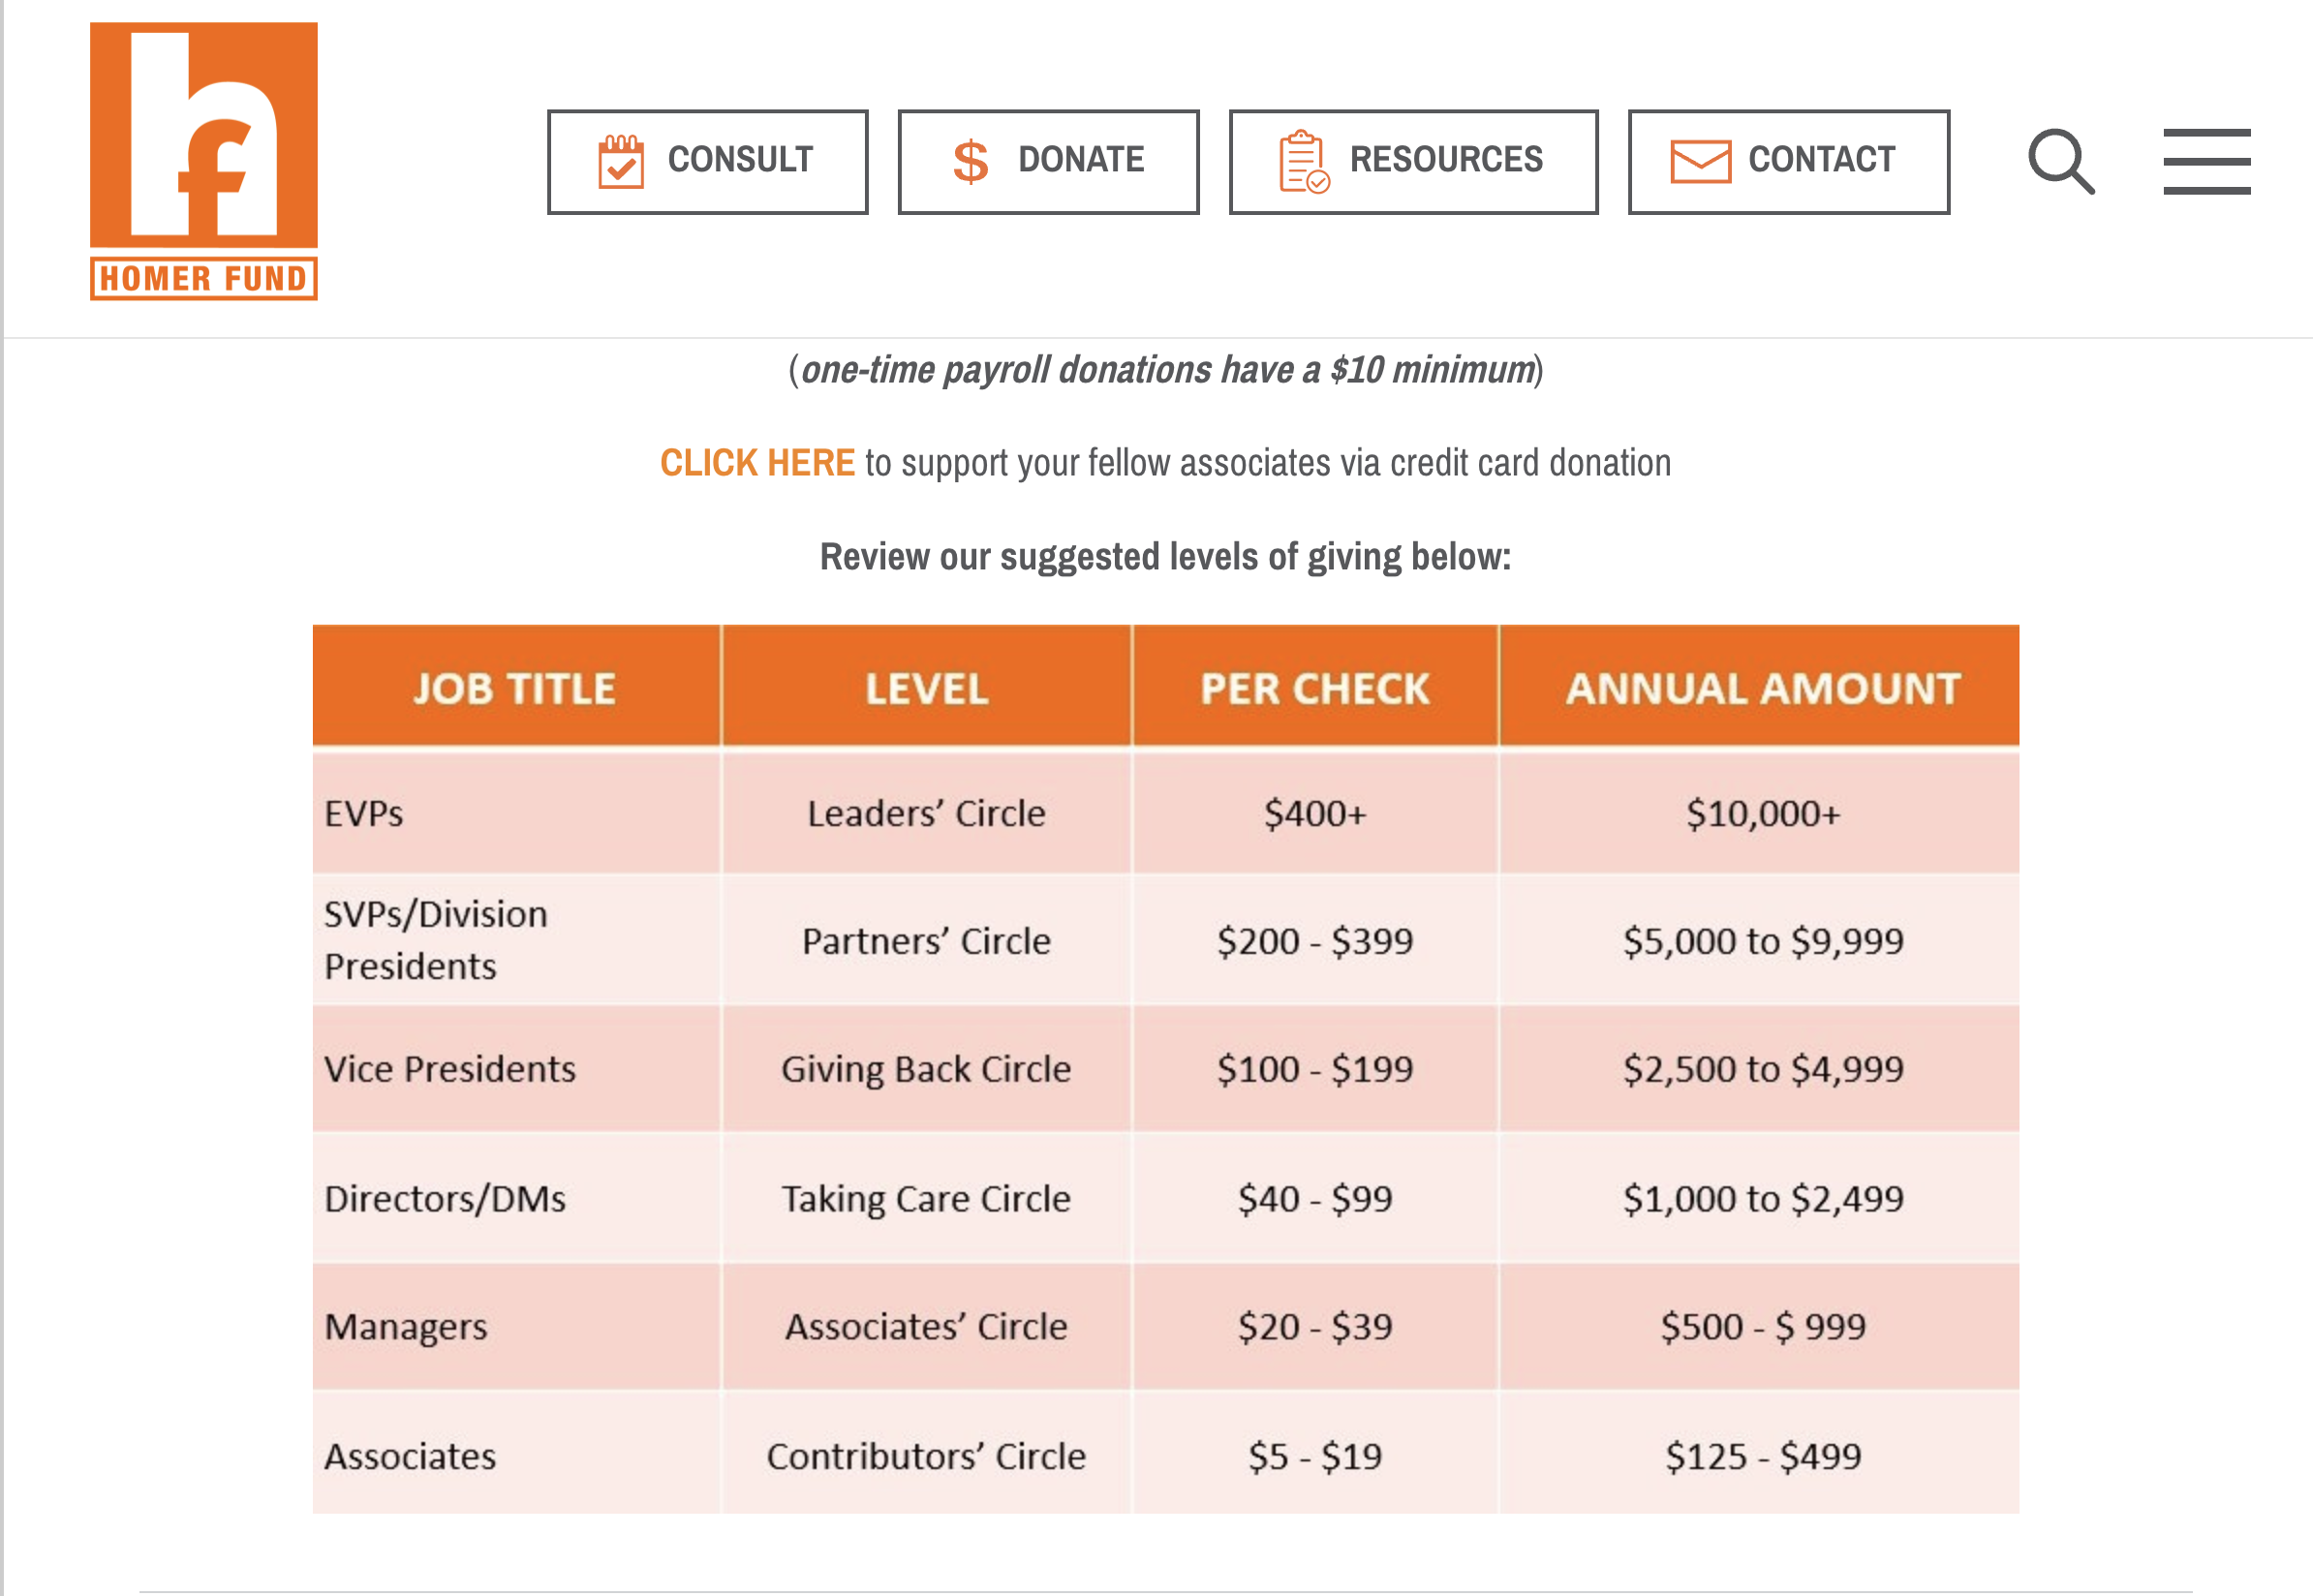
\includegraphics[width=0.6\linewidth]{../plots/HF_donation_suggestions} \caption{Suggested Homer Fund donation levels as of 2025}\label{fig:fig-sugdon}
\end{figure}

\FloatBarrier
\newpage

\section{Home Depot Survey summary table (unweighted)}\label{app-survsum-uw}

The unweighted sample is older and skewed slightly male relative to reported Facebook demographics for Home Depot workers.\footnote{Our sample is 56\% male and has a median age of 50 compared to Facebook reported values of 53\% male with a median age in the 30-39 interval. The weighted sample is 52\% male with a median age of 38.} The sample is 79\% white.

\begin{table}

\caption{\label{tab:tab-sum-uw}\textbf{Sample summary statistics by treatment group}}
\centering
\begin{tabular}[t]{l|c|c|c}
\hline
\textbf{Characteristic} & \makecell[c]{\textbf{cntrl}\ \ \\N = 164} & \makecell[c]{\textbf{txt}\ \ \\N = 197} & \makecell[c]{\textbf{vid}\ \ \\N = 154}\\
\hline
\textbf{EHF awareness (list)} & 98 (60\%) & 120 (61\%) & 94 (61\%)\\
\hline
\textbf{EHF awareness (cntrl)} &  &  & \\
\hline
\hspace{1em}Don’t know & 17 (10\%) & 0 (NA\%) & 0 (NA\%)\\
\hline
\hspace{1em}No & 9 (5.5\%) & 0 (NA\%) & 0 (NA\%)\\
\hline
\hspace{1em}Yes & 138 (84\%) & 0 (NA\%) & 0 (NA\%)\\
\hline
\hspace{1em}(missing/not gathered) & 0 & 197 & 154\\
\hline
\textbf{age} & 52 (31, 62) & 47 (32, 61) & 51 (34, 62)\\
\hline
\textbf{male} & 98 (60\%) & 109 (56\%) & 81 (53\%)\\
\hline
\hspace{1em}(missing/not gathered) & 0 & 1 & 1\\
\hline
\textbf{main job} & 147 (90\%) & 176 (89\%) & 139 (90\%)\\
\hline
\hspace{1em}(missing/not gathered) & 1 & 0 & \vphantom{1} 0\\
\hline
\textbf{job tenure} &  &  & \\
\hline
\hspace{1em}Less than 6 months & 10 (6.1\%) & 13 (6.6\%) & 7 (4.5\%)\\
\hline
\hspace{1em}At least 6 months but less than 1 year & 16 (9.8\%) & 8 (4.1\%) & 12 (7.8\%)\\
\hline
\hspace{1em}At least 1 year but less than 2 years & 25 (15\%) & 25 (13\%) & 30 (19\%)\\
\hline
\hspace{1em}At least 2 years but less than 3 years & 15 (9.1\%) & 15 (7.6\%) & 16 (10\%)\\
\hline
\hspace{1em}3 or more years & 98 (60\%) & 136 (69\%) & 89 (58\%)\\
\hline
\textbf{PoC/nonwhite} & 38 (23\%) & 33 (17\%) & 37 (24\%)\\
\hline
\hspace{1em}(missing/not gathered) & 1 & 3 & 1\\
\hline
\textbf{full time} & 98 (60\%) & 138 (70\%) & 91 (59\%)\\
\hline
\textbf{hourly} & 158 (96\%) & 186 (94\%) & 153 (99\%)\\
\hline
\textbf{college degree} & 37 (23\%) & 43 (22\%) & 29 (19\%)\\
\hline
\textbf{knows EHF recipient} & 0 (NA\%) & 120 (61\%) & 82 (53\%)\\
\hline
\hspace{1em}(missing/not gathered) & 164 & 1 & 0\\
\hline
\textbf{applied to EHF} & 0 (NA\%) & 45 (23\%) & 35 (23\%)\\
\hline
\hspace{1em}(missing/not gathered) & 164 & 0 & 0\\
\hline
\textbf{received EHF grant} & 22 (13\%) & 27 (14\%) & 22 (14\%)\\
\hline
\textbf{donated to EHF} &  &  & \\
\hline
\hspace{1em}Don’t know & 7 (4.3\%) & 6 (3.0\%) & 11 (7.1\%)\\
\hline
\hspace{1em}No & 36 (22\%) & 25 (13\%) & 33 (21\%)\\
\hline
\hspace{1em}Yes & 120 (74\%) & 166 (84\%) & 110 (71\%)\\
\hline
\hspace{1em}(missing/not gathered) & 1 & 0 & 0\\
\hline
\multicolumn{4}{l}{\rule{0pt}{1em}\textsuperscript{1} n (\%); Median (Q1, Q3)}\\
\end{tabular}
\end{table}

\begin{table}

\caption{\label{tab:tab-sum-uw}\textit{summary table (cont'd)}}
\centering
\begin{tabular}[t]{l|c|c|c}
\hline
\textbf{Characteristic} & \makecell[c]{\textbf{cntrl}\ \ \\N = 164} & \makecell[c]{\textbf{txt}\ \ \\N = 197} & \makecell[c]{\textbf{vid}\ \ \\N = 154}\\
\hline
\textbf{loyalty to coworkers} &  &  & \\
\hline
\hspace{1em}No loyalty at all & 14 (8.6\%) & 10 (5.1\%) & 6 (3.9\%)\\
\hline
\hspace{1em}Only a little loyalty & 16 (9.8\%) & 27 (14\%) & 11 (7.1\%)\\
\hline
\hspace{1em}Some loyalty & 65 (40\%) & 83 (42\%) & 52 (34\%)\\
\hline
\hspace{1em}A lot of loyalty & 68 (42\%) & 77 (39\%) & 85 (55\%)\\
\hline
\hspace{1em}(missing/not gathered) & 1 & 0 & 0\\
\hline
\textbf{loyalty to employer} &  &  & \\
\hline
\hspace{1em}No loyalty at all & 23 (14\%) & 22 (11\%) & 8 (5.2\%)\\
\hline
\hspace{1em}Only a little loyalty & 25 (16\%) & 27 (14\%) & 24 (16\%)\\
\hline
\hspace{1em}Some loyalty & 45 (28\%) & 81 (42\%) & 44 (29\%)\\
\hline
\hspace{1em}A lot of loyalty & 67 (42\%) & 65 (33\%) & 77 (50\%)\\
\hline
\hspace{1em}(missing/not gathered) & 4 & 2 & 1\\
\hline
\textbf{recommend employer} &  &  & \\
\hline
\hspace{1em}Definitely would not recommend & 24 (15\%) & 20 (10\%) & 6 (3.9\%)\\
\hline
\hspace{1em}Might not recommend & 11 (6.7\%) & 21 (11\%) & 10 (6.5\%)\\
\hline
\hspace{1em}Not sure & 10 (6.1\%) & 16 (8.2\%) & 9 (5.8\%)\\
\hline
\hspace{1em}Might recommend & 34 (21\%) & 46 (23\%) & 43 (28\%)\\
\hline
\hspace{1em}Certainly would recommend & 85 (52\%) & 93 (47\%) & 86 (56\%)\\
\hline
\hspace{1em}(missing/not gathered) & 0 & 1 & 0\\
\hline
\textbf{union vote} &  &  & \\
\hline
\hspace{1em}Against the union & 78 (48\%) & 99 (50\%) & 66 (43\%)\\
\hline
\hspace{1em}For the union & 41 (25\%) & 43 (22\%) & 24 (16\%)\\
\hline
\hspace{1em}Not sure & 45 (27\%) & 55 (28\%) & 63 (41\%)\\
\hline
\hspace{1em}(missing/not gathered) & 0 & 0 & 1\\
\hline
\textbf{UI support} &  &  & \\
\hline
\hspace{1em}No responsibility & 34 (21\%) & 31 (16\%) & 14 (9.2\%)\\
\hline
\hspace{1em}A little responsibility & 39 (24\%) & 53 (27\%) & 37 (24\%)\\
\hline
\hspace{1em}Some responsibility & 52 (32\%) & 57 (29\%) & 51 (33\%)\\
\hline
\hspace{1em}A lot of responsibility & 39 (24\%) & 53 (27\%) & 51 (33\%)\\
\hline
\hspace{1em}(missing/not gathered) & 0 & 3 & 1\\
\hline
\textbf{pension support} &  &  & \\
\hline
\hspace{1em}No responsibility & 17 (10\%) & 18 (9.3\%) & 9 (5.9\%)\\
\hline
\hspace{1em}A little responsibility & 17 (10\%) & 23 (12\%) & 13 (8.6\%)\\
\hline
\hspace{1em}Some responsibility & 40 (25\%) & 60 (31\%) & 44 (29\%)\\
\hline
\hspace{1em}A lot of responsibility & 88 (54\%) & 93 (48\%) & 86 (57\%)\\
\hline
\hspace{1em}(missing/not gathered) & 2 & 3 & 2\\
\hline
\textbf{childcare support} &  &  & \\
\hline
\hspace{1em}No responsibility & 36 (22\%) & 37 (19\%) & 24 (16\%)\\
\hline
\hspace{1em}A little responsibility & 29 (18\%) & 28 (15\%) & 20 (13\%)\\
\hline
\hspace{1em}Some responsibility & 48 (29\%) & 76 (39\%) & 64 (42\%)\\
\hline
\hspace{1em}A lot of responsibility & 50 (31\%) & 52 (27\%) & 43 (28\%)\\
\hline
\hspace{1em}(missing/not gathered) & 1 & 4 & 3\\
\hline
\multicolumn{4}{l}{\rule{0pt}{1em}\textsuperscript{1} n (\%)}\\
\end{tabular}
\end{table}

\FloatBarrier
\newpage

\section{Walmart Survey summary table (unweighted)}\label{app-wmt-survsum}

\begin{table}

\caption{\label{tab:tab-sum-wmt}\textbf{Sample summary statistics by treatment group}}
\centering
\begin{tabular}[t]{l|c|c|c|c}
\hline
\textbf{Characteristic} & \makecell[c]{\textbf{ctrl}\ \ \\N = 260} & \makecell[c]{\textbf{vid0}\ \ \\N = 254} & \makecell[c]{\textbf{vidChar}\ \ \\N = 237} & \makecell[c]{\textbf{vidSolid}\ \ \\N = 229}\\
\hline
\textbf{EHF awareness (pre-treatment)} & 116 (45\%) & 97 (38\%) & 91 (38\%) & 85 (37\%)\\
\hline
\textbf{age} &  &  &  & \\
\hline
\hspace{1em}18-45 & 115 (44\%) & 114 (45\%) & 132 (56\%) & 103 (45\%)\\
\hline
\hspace{1em}45-65+ & 145 (56\%) & 140 (55\%) & 105 (44\%) & 126 (55\%)\\
\hline
\textbf{male} & 55 (21\%) & 55 (22\%) & 63 (27\%) & 47 (21\%)\\
\hline
\textbf{main job} & 224 (86\%) & 232 (91\%) & 207 (87\%) & 205 (90\%)\\
\hline
\textbf{job tenure} &  &  &  & \\
\hline
\hspace{1em}3 or more years & 124 (48\%) & 129 (51\%) & 116 (49\%) & 106 (46\%)\\
\hline
\hspace{1em}At least 1 year but less than 2 years & 49 (19\%) & 43 (17\%) & 41 (17\%) & 46 (20\%)\\
\hline
\hspace{1em}At least 2 years but less than 3 years & 25 (9.6\%) & 27 (11\%) & 24 (10\%) & 24 (10\%)\\
\hline
\hspace{1em}At least 6 months but less than 1 year & 32 (12\%) & 26 (10\%) & 27 (11\%) & 23 (10\%)\\
\hline
\hspace{1em}Less than 6 months & 30 (12\%) & 29 (11\%) & 29 (12\%) & 30 (13\%)\\
\hline
\textbf{PoC/nonwhite} & 51 (20\%) & 49 (19\%) & 52 (22\%) & 39 (17\%)\\
\hline
\textbf{full time} & 196 (75\%) & 193 (76\%) & 187 (79\%) & 189 (83\%)\\
\hline
\textbf{hourly} & 248 (95\%) & 247 (97\%) & 227 (96\%) & 223 (97\%)\\
\hline
\textbf{college degree} & 24 (9.2\%) & 25 (9.8\%) & 18 (7.6\%) & 23 (10\%)\\
\hline
\textbf{EHF awareness (post-treatment)} &  &  &  & \\
\hline
\hspace{1em}No & 98 (56\%) & 109 (61\%) & 98 (54\%) & 107 (56\%)\\
\hline
\hspace{1em}Unsure & 14 (8.0\%) & 15 (8.4\%) & 8 (4.4\%) & 17 (8.9\%)\\
\hline
\hspace{1em}Yes & 63 (36\%) & 54 (30\%) & 75 (41\%) & 67 (35\%)\\
\hline
\hspace{1em}(missing/not gathered) & 85 & 76 & 56 & \vphantom{2} 38\\
\hline
\textbf{applied to EHF} &  &  &  & \\
\hline
\hspace{1em}Don't know & 4 (2.3\%) & 4 (2.2\%) & 3 (1.7\%) & 0 (0\%)\\
\hline
\hspace{1em}No & 143 (82\%) & 155 (87\%) & 149 (82\%) & 168 (88\%)\\
\hline
\hspace{1em}Yes & 28 (16\%) & 19 (11\%) & 29 (16\%) & 23 (12\%)\\
\hline
\hspace{1em}(missing/not gathered) & 85 & 76 & 56 & \vphantom{1} 38\\
\hline
\textbf{received EHF grant} & 19 (59\%) & 8 (35\%) & 18 (56\%) & 14 (61\%)\\
\hline
\hspace{1em}(missing/not gathered) & 228 & 231 & 205 & 206\\
\hline
\textbf{donated to EHF} & 16 (9.1\%) & 15 (8.4\%) & 29 (16\%) & 18 (9.4\%)\\
\hline
\hspace{1em}(missing/not gathered) & 85 & 76 & 56 & 38\\
\hline
\multicolumn{5}{l}{\rule{0pt}{1em}\textsuperscript{1} n (\%)}\\
\end{tabular}
\end{table}

\begin{table}

\caption{\label{tab:tab-sum-wmt}\textit{summary table (cont'd)}}
\centering
\begin{tabular}[t]{l|c|c|c|c}
\hline
\textbf{Characteristic} & \makecell[c]{\textbf{ctrl}\ \ \\N = 260} & \makecell[c]{\textbf{vid0}\ \ \\N = 254} & \makecell[c]{\textbf{vidChar}\ \ \\N = 237} & \makecell[c]{\textbf{vidSolid}\ \ \\N = 229}\\
\hline
\textbf{loyalty to coworkers} &  &  &  & \\
\hline
\hspace{1em}A lot of loyalty & 72 (28\%) & 85 (33\%) & 77 (32\%) & 76 (33\%)\\
\hline
\hspace{1em}No loyalty at all & 29 (11\%) & 15 (5.9\%) & 22 (9.3\%) & 19 (8.3\%)\\
\hline
\hspace{1em}Only a little loyalty & 43 (17\%) & 48 (19\%) & 36 (15\%) & 42 (18\%)\\
\hline
\hspace{1em}Some loyalty & 116 (45\%) & 106 (42\%) & 102 (43\%) & 92 (40\%)\\
\hline
\textbf{loyalty to employer} &  &  &  & \\
\hline
\hspace{1em}A lot of loyalty & 62 (24\%) & 72 (28\%) & 57 (24\%) & 65 (28\%)\\
\hline
\hspace{1em}No loyalty at all & 65 (25\%) & 55 (22\%) & 46 (19\%) & 49 (21\%)\\
\hline
\hspace{1em}Only a little loyalty & 50 (19\%) & 51 (20\%) & 51 (22\%) & 49 (21\%)\\
\hline
\hspace{1em}Some loyalty & 83 (32\%) & 76 (30\%) & 83 (35\%) & 66 (29\%)\\
\hline
\textbf{recommend employer} &  &  &  & \\
\hline
\hspace{1em}Certainly would recommend & 90 (35\%) & 97 (38\%) & 80 (34\%) & 80 (35\%)\\
\hline
\hspace{1em}Definitely would not recommend & 44 (17\%) & 31 (12\%) & 33 (14\%) & 34 (15\%)\\
\hline
\hspace{1em}Might not recommend & 31 (12\%) & 29 (11\%) & 34 (14\%) & 30 (13\%)\\
\hline
\hspace{1em}Might recommend & 72 (28\%) & 72 (28\%) & 75 (32\%) & 57 (25\%)\\
\hline
\hspace{1em}Not sure & 23 (8.8\%) & 25 (9.8\%) & 15 (6.3\%) & 28 (12\%)\\
\hline
\textbf{union vote} &  &  &  & \\
\hline
\hspace{1em}Against the union & 50 (19\%) & 40 (16\%) & 29 (12\%) & 29 (13\%)\\
\hline
\hspace{1em}For the union & 113 (43\%) & 112 (44\%) & 117 (49\%) & 103 (45\%)\\
\hline
\hspace{1em}Leaning against voting for the union & 7 (2.7\%) & 4 (1.6\%) & 4 (1.7\%) & 3 (1.3\%)\\
\hline
\hspace{1em}Leaning toward voting for the union & 7 (2.7\%) & 11 (4.3\%) & 5 (2.1\%) & 6 (2.6\%)\\
\hline
\hspace{1em}Not sure & 83 (32\%) & 87 (34\%) & 82 (35\%) & 88 (38\%)\\
\hline
\textbf{hardship support} &  &  &  & \\
\hline
\hspace{1em}A little responsibility & 30 (12\%) & 37 (15\%) & 36 (15\%) & 24 (10\%)\\
\hline
\hspace{1em}A lot of responsibility & 105 (40\%) & 117 (46\%) & 104 (44\%) & 109 (48\%)\\
\hline
\hspace{1em}No responsibility & 15 (5.8\%) & 11 (4.3\%) & 7 (3.0\%) & 5 (2.2\%)\\
\hline
\hspace{1em}Some responsibility & 110 (42\%) & 89 (35\%) & 90 (38\%) & 91 (40\%)\\
\hline
\textbf{pension support} &  &  &  & \\
\hline
\hspace{1em}A little responsibility & 10 (3.8\%) & 8 (3.1\%) & 13 (5.5\%) & 11 (4.8\%)\\
\hline
\hspace{1em}A lot of responsibility & 192 (74\%) & 192 (76\%) & 175 (74\%) & 180 (79\%)\\
\hline
\hspace{1em}No responsibility & 5 (1.9\%) & 2 (0.8\%) & 2 (0.8\%) & 5 (2.2\%)\\
\hline
\hspace{1em}Some responsibility & 53 (20\%) & 52 (20\%) & 47 (20\%) & 33 (14\%)\\
\hline
\textbf{UI support} &  &  &  & \\
\hline
\hspace{1em}A little responsibility & 35 (13\%) & 49 (19\%) & 46 (19\%) & 30 (13\%)\\
\hline
\hspace{1em}A lot of responsibility & 92 (35\%) & 97 (38\%) & 82 (35\%) & 95 (41\%)\\
\hline
\hspace{1em}No responsibility & 21 (8.1\%) & 13 (5.1\%) & 8 (3.4\%) & 11 (4.8\%)\\
\hline
\hspace{1em}Some responsibility & 112 (43\%) & 95 (37\%) & 101 (43\%) & 93 (41\%)\\
\hline
\multicolumn{5}{l}{\rule{0pt}{1em}\textsuperscript{1} n (\%)}\\
\end{tabular}
\end{table}

\newpage

\section{Alternative specifications \& Study 1}\label{alternative-specifications-study-1}

\section{Alternative specifications \& Study 2}\label{alternative-specifications-study-2}

\section{Video treatment and placebo similarities}\label{app-vidsim}

We use text, acoustic, and dynamic video embeddings to characterize the multimodal similarity between (i) the Walmart placebo and treatment videos and (ii) the Home Depot and Walmart treatment videos. Visual comparability is assessed with CLIP ViT-B/32 (\citeproc{ref-radfordLearningTransferableVisual2021}{\textbf{radfordLearningTransferableVisual2021?}}), implemented via OpenCLIP on 200 frames per file. For acoustic similarity, we segment the audio tracks into overlapping 10-second windows and encode them with CLAP (\citeproc{ref-wuLargeScaleContrastiveLanguageAudio2023}{\textbf{wuLargeScaleContrastiveLanguageAudio2023?}}). For transcript comparability we use Sentence-BERT embeddings (\citeproc{ref-reimersSentenceBERTSentenceEmbeddings2019}{\textbf{reimersSentenceBERTSentenceEmbeddings2019?}}) to capture semantic similarity of the narrated content. In each case we report the cosine similarity of the mean embeddings as the video-level score.

The results match the design. The placebo and treatment videos are highly similar in visual and acoustic form but diverge sharply in semantic content, isolating message content from audiovisual style. The Home Depot and Walmart treatment videos, by contrast, are highly similar across all three modalities---visual, acoustic, and semantic---confirming that the Walmart-adapted video is a faithful analog of the Homer Fund original.

\begin{figure}[H]

{\centering \includegraphics[width=0.8\linewidth]{../plots/compare_charity_placebo_summary} 

}

\caption{Multimodal similarity: Walmart treatment vs. Walmart placebo}\label{fig:unnamed-chunk-1}
\end{figure}

\begin{figure}[H]

{\centering \includegraphics[width=0.8\linewidth]{../plots/compare_trt_charity_summary} 

}

\caption{Multimodal similarity: Home Depot treatment vs. Walmart treatment}\label{fig:unnamed-chunk-2}
\end{figure}

\newpage

\section{Manipulation check Study 3}\label{app-wmt-manip}

In the Walmart sample, treatment significantly increased the probability that a respondent would correctly state that Walmart has an EHF.

\begin{table}[H]
\centering\centering
\caption{\label{tab:setup}OLS regression of treatment on correctly reporting a Walmart EHF (manipulation check) \label{tab:tab-manip-check}}
\centering
\begin{threeparttable}
\begin{tabular}[t]{lcccc}
\toprule
  & (1) & (2) & (3) & (4)\\
\midrule
treated & \num{0.118}*** &  & \num{0.103}*** & \\
 & (\num{0.029}) &  & (\num{0.028}) & \\
placebo &  & \num{-0.061} &  & \num{-0.027}\\
 &  & (\num{0.037}) &  & (\num{0.032})\\
charity treatment &  & \num{0.097}** &  & \num{0.067}*\\
 &  & (\num{0.041}) &  & (\num{0.040})\\
solidarity treatment &  & \num{0.079}* &  & \num{0.111}***\\
 &  & (\num{0.042}) &  & (\num{0.042})\\
pre-exposed &  &  & \num{0.349}*** & \num{0.360}***\\
 &  &  & (\num{0.038}) & (\num{0.053})\\
treat x pre-exposed &  &  & \num{0.073} & \\
 &  &  & (\num{0.058}) & \\
placebo x pre-exposed &  &  &  & \num{-0.028}\\
 &  &  &  & (\num{0.076})\\
charity x pre-exposed &  &  &  & \num{0.135}*\\
 &  &  &  & (\num{0.079})\\
solidarity x pre-exposed &  &  &  & \num{-0.015}\\
 &  &  &  & (\num{0.083})\\
\midrule
$N$ & \num{980} & \num{980} & \num{980} & \num{980}\\
\bottomrule
\end{tabular}
\begin{tablenotes}
\item * p $<$ 0.1, ** p $<$ 0.05, *** p $<$ 0.01 Robust standard errors in parentheses.
\end{tablenotes}
\end{threeparttable}
\end{table}

\newpage

\section{Alternative models for ACNT donation}\label{app-wmt-altdonate}

\begin{table}[H]
\centering\centering
\caption{\label{tab:fig-emerg-donate}Regression of ACNT donation on treatment  \label{tab:tab-donate-models-wmt-app}}
\centering
\begin{threeparttable}
\begin{tabular}[t]{lccc}
\toprule
  & LPM & logit & Firth\\
\midrule
Treated & \num{0.038}** & \num{0.440}** & \num{0.437}**\\
 & (\num{0.019}) & (\num{0.219}) & (\num{0.218})\\
\midrule
N & \num{980} & \num{980} & \num{980}\\
AIC & \num{386.8} & \num{619.3} & \\
\bottomrule
\end{tabular}
\begin{tablenotes}
\item * p $<$ 0.1, ** p $<$ 0.05, *** p $<$ 0.01 Robust standard errors for OLS model
\end{tablenotes}
\end{threeparttable}
\end{table}

\newpage

\section{Alternative specifications \& Study 3}\label{alternative-specifications-study-3}

\newpage

\section{Placebos for UI support (Home Depot)}\label{app-placebo}

\begin{table}[H]
\centering\centering
\caption{\label{tab:fig-ui}Support for other social policies, OLS regression  \label{tab:tab-placebo}}
\centering
\begin{threeparttable}
\begin{tabular}[t]{lcc}
\toprule
  & Pension & Childcare\\
\midrule
Text treatment & \num{-0.031} & \num{-0.028}\\
 & (\num{0.060}) & (\num{0.066})\\
Video treatment & \num{0.052} & \num{-0.031}\\
 & (\num{0.057}) & (\num{0.068})\\
Pre-exposed & \num{0.007} & \num{-0.028}\\
 & (\num{0.055}) & (\num{0.061})\\
Text x pre-exposed & \num{0.022} & \num{0.076}\\
 & (\num{0.074}) & (\num{0.082})\\
Video x pre-exposed & \num{-0.013} & \num{0.133}\\
 & (\num{0.073}) & (\num{0.085})\\
\midrule
$N$ & \num{508} & \num{507}\\
$R^2$ & \num{0.01} & \num{0.01}\\
AIC & \num{290.5} & \num{400.2}\\
\bottomrule
\end{tabular}
\begin{tablenotes}
\item * p $<$ 0.1, ** p $<$ 0.05, *** p $<$ 0.01 Robust standard errors in parentheses.
\end{tablenotes}
\end{threeparttable}
\end{table}

\end{document}
